\documentclass[preprint,5p,times]{elsarticle}
\undef{\Bbbk}
\usepackage{todo}
\usepackage{verbatim}
\usepackage{fancyvrb}
\usepackage{adjustbox}
\usepackage{xurl}
\usepackage{setspace}
\usepackage{listings}
\usepackage{svg}
\usepackage{pifont}
\usepackage{breakurl}
\usepackage{makecell}

\definecolor{OrangeGSSI}{RGB}{237,113,45}
\definecolor{blue}{RGB}{25,25,112}
\definecolor{ashgrey}{rgb}{0.85, 0.85, 0.85}
\usepackage{tikz}
\usetikzlibrary{arrows,shadows}
\usepackage{pgf-umlsd}
\usepackage{pgfplots}
\pgfplotsset{height=8.5cm,width=1.8\linewidth,compat=1.15}
\usepackage{subfig}
\usepackage{placeins}

%Sequence Diagram Packages

\usepackage{float}
\usepackage{pifont}
\usepackage{xcolor,colortbl}
\usepackage{flushend}
\usepackage[normalem]{ulem} % for \sout
\usepackage{multicol}

\usepackage{pifont}
\newcommand{\cmark}{\textcolor{black}{\ding{51}}}
\newcommand{\xmark}{\textcolor{black}{\ding{55}}}
\usepackage[acronym,automake,nopostdot,nonumberlist]{glossaries}
\usepackage[subtle]{savetrees}

\usepackage{titlesec}
\titlespacing\section{0pt}{12pt plus 4pt minus 2pt}{0pt plus 2pt minus 2pt}
\titlespacing\subsection{0pt}{12pt plus 4pt minus 2pt}{0pt plus 2pt minus 2pt}
\titlespacing\subsubsection{0pt}{12pt plus 4pt minus 2pt}{0pt plus 2pt minus 2pt}
\makeglossaries	

\newacronym{iot}{IoT}{Internet of Things}
\newacronym{ics}{ICS}{Industrial Control System}
\newacronym{ot}{OT}{Operation Technology}
\newacronym{plc}{PLC}{Programmable Logic Controller}
\newacronym{dcs}{DCS}{Distributed Control System}
\newacronym{scada}{SCADA}{Supervisory Control and Data Acquisition}
\newacronym{ci}{CI}{Critical Infrastructures}
\newacronym{cps}{CPS}{Cyber-Physical System}
\newacronym{gui}{GUI}{Graphical User Interface}
\newacronym{iiot}{IIoT}{Industrial Internet of Things}
\newacronym{nse}{NSE}{Nmap Scripting Engine}
\newacronym{osi}{OSI}{Open Systems Interconnection}
\newacronym{mqtt}{MQTT}{Message Queue Telemetry Transport}
\newacronym{amqp}{AMQP}{Advanced Message Queuing Protocol}
\newacronym{oasis}{OASIS}{Organization for the Advancement of Structured Information Standards}
\newacronym{coap}{CoAP}{Constrained Application Protocol}
\newacronym{adu}{ADU}{Application Data Unit}
\newacronym{pdu}{PDU}{Protocol Data Unit}
\newacronym{mbap}{MBAP}{MODBUS Application}
\newacronym{isotsap}{ISO-TSAP}{ISO Transport Service on top of TCP}
\newacronym{mitm}{MITM}{Man in the Middle}
\newacronym{xml}{XML}{Extensible Markup Language}
\newacronym{cli}{CLI}{Command Line Interface}
\newacronym{bpf}{BPF}{Berkley Packer Filter}
\newacronym{tpkt}{TPKT}{Transport Packet}
\newacronym{cotp}{COTP}{Connection-Oriented Transport}

\newcommand{\rotation}[3][20em]{% \turn[<width>]{<angle>}{<stuff>}
	\rlap{\rotatebox{#2}{\begin{varwidth}[t]{#1}\bfseries#3\end{varwidth}}}%
}

\usepackage{amsthm}

\newtheorem{remark}{Remark}


\undef{\Bbbk}

\lstset{
  inputencoding=utf8,
  columns=flexible,
  keepspaces=true,
  showstringspaces=false,
  basicstyle=\tiny\ttfamily,
  commentstyle=\color{gray},
  keywordstyle=\color{purple},
  stringstyle=\color{green}
}



\lstset{captionpos=b,
    frame=tb,
    basicstyle=\scriptsize\ttfamily,
    showstringspaces=false,
    keepspaces=true}

	 

\begin{document}
	
\begin{frontmatter}

\title{LOGistICS: A Medium-Interaction Emulation and Monitoring System for Operational Technology}

\author[unipg]{Stefano~Bistarelli}
\ead{stefano.bistarelli@unipg.it}
\author[unipg]{Emanuele~Bosimini}
\ead{emanuelebosimini@gmail.com}
\author[unipg]{Francesco~Santini
	\corref{cor1}}
\ead{francesco.santini@dmi.unipg.it}


%\cortext[cor1]{Partially supported by the MIUR PRIN 2017FTXR7S ``IT-MaTTerS''.}
\cortext[cor1]{Corresponding author.}

\address[unipg]{Dipartimento di Matematica e Informatica, Universit\`a degli Studi di Perugia, Perugia, Italy}

%\author{Stefano Bistarelli}
%\affiliation{%
%	\institution{Dip. Matematica e Informatica \\Universit{\`a} degli Studi di Perugia}
%	\streetaddress{Via Vanvitelli 1}
%	\city{Perugia}
%	\country{Italy}}
%\email{stefano.bistarelli@unipg.it}

%\author{Emanuele Bosimini}
%\affiliation{%
% \institution{Dip. Matematica e Informatica \\ Universit{\`a} degli Studi di Perugia}
% \streetaddress{Via Vanvitelli 1}
% \city{Perugia}
% \country{Italy}}
%\email{emanuele.bosimini@studenti.unipg.it}

%\author{Francesco Santini}
%\affiliation{%
%	\institution{Dip. Matematica e Informatica \\ Universit{\`a} degli Studi di Perugia}
%	\streetaddress{Via Vanvitelli 1}
%	\city{Perugia}
%	\country{Italy}}
%\email{francesco.santini@unipg.it}




\begin{abstract}
We present LOGistICS, a novel monitoring-framework with the aim to study the security of industrial PLC systems. The architecture encompasses different processing components and probes, with different tasks. In particular, this paper focuses on the description of a new medium-interaction honeypot attracting Modbus and S7comm traffic. We analyze this honeypot in deep by presenting different experiments, among which leaving them open to the Internet for a couple of months. With respect to related open-projects, our proposal is highly extensible, configurable, and it allows for interacting more with an attacker while remaining less detectable.
\end{abstract}



\begin{keyword}
Honeypot, ICS, S7comm, Modbus
\end{keyword}

\end{frontmatter}

\section{Introduction}\label{sect:intro}
\emph{Industrial Control Systems} (\acrshort{ics})~\cite{ICS} are command and control networks and systems designed to support industrial processes. These systems also operate critical infrastructures, such as electricity generation plants, transportation systems, oil refineries, chemical factories and manufacturing facilities: hence, protecting the is crucial for the safety of citizens.
\emph{Operational Technology} (\acrshort{ot}) is a term that collectively concern hardware and software that detects or causes a change through the direct monitoring and/or control of physical devices, processes and events in such systems. Examples are \emph{Supervisory Control and Data Acquisition} (\acrshort{scada}) and \emph{Programming Logic Controllers} (\acrshort{plc}). 

Initially, \acrshort{ics} were isolated by nature~\cite{ICS}, being limited to the process network.
Security was ensured by both obscurity and isolation.
The protocols were proprietary and related documentation was not publicly available.
We could forcefully say that the systems, not being connected to the internet, were safer.
However, nowadays, in the era of Industry 4.0, \acrshort{ics} are able to be interconnected in a production intranet, and consequently exposed to the Internet through the company network.
This need for connection, also combining the questionable paradigm of making
open standards, clearly exposes \acrshort{ics} to serious safety problems.

We can think about resorting to protection measures adopted in conventional ICT systems, such as a Firewall or an Intrusion Detection System.
However, this introduces design-related safety issues. The priority of an ICT system is to focus on confidentiality and data integrity, but,
on the other hand, \acrshort{ics} are designed to ensure \emph{reliability/availability}, even jeopardizing the \emph{confidentiality} and \emph{integrity} of data. Further common goals in ICS are related to the \emph{safety} of operators and environment, and, of course, \emph{productivity}.
An example of such different security concerns with respect to ICT systems is represented by the Modbus protocol~\cite{modbustcp}, a long-lived and reliable protocol, which nonetheless comes without authentication mechanisms.

Nowadays the devices and protocols adopted in an ICS are used in nearly every industrial sector and critical infrastructure such as the manufacturing, transportation, energy, and water treatment industries.
Given all the introduced peculiarities and the importance of monitoring security in such applications, in this paper we present \emph{LOGistICS}, an emulation and monitoring system for~\acrshort{ot}. In particular, we focus on two typical ICS protocols, such as S7comm from Siemens~\cite{xiao2017s7commtrace} and Modbus from Schneider Electric~\cite{modbustcp}, 
which are also used extensively in home and building automation.
The framework we propose is composed of \emph{i)} a highly customizable \emph{honeypot} that emulates the two aforementioned ICS services,
\emph{ii)} a sniffer that records traffic, and \emph{iii)} a monitoring node, which is capable of analyzing and plotting recorded data. A fourth component implements malicious activities towards the honeypots, being an attacking node not properly part of the monitoring platform (more a test node).

Among all these components, this paper mainly focuses on Modbus  and S7comm honeypots. What described in the following  goes under the umbrella of \emph{deception technology}, which is an emerging category of cybersecurity defense. Deception technology automates the creation of traps (decoys), and can detect, analyze, and defend against zero-day and advanced attacks, often in real time.

Honeypots~\cite{survey1} are hardware/software components used as ``baits'' to attract attackers: their purpose is to expose only the vulnerable interface of a complete service (e.g., Telnet), without implementing all their logic and functionality. Honeypots can therefore be used to attract and record attacks by identifying the underlying patterns. A widely used classification of honeypots is based upon the characteristics of interaction. Low-interaction honeypots produce minimal responses in order to allow protocol handshakes: they are used mainly for statistic evaluation, and they suffice to recognize peaks in the number of requests, for example created by autonomous malware.
Medium interaction honeypots are more elaborated and provide a higher level of interaction for the attacker: their goal is to produce reasonable replies in hope of triggering follow-up attacks. In other hand, high-interaction honeypots, exposing additional resources than the previous ones, collect the largest possible amount of information, including complete attack logs, data access, traversing of file trees, executed byte codes, etc.

LOGistICS is light, stealthy, isolated through containerization technologies, cross-platform, easy to deploy, with a fair degree of interaction.
Our honeypots system is based on two libraries that allow communication via S7comm and Modbus protocols: \emph{Snap7}\footnote{Snap7: \url{http://snap7.sourceforge.net}.} and \emph{Pymodbus}\footnote{Pymodbus: \url{https://pymodbus.readthedocs.io/en/latest/}.} respectively.
With the purpose to deceive search engines, we made some low-level changes to make the behavior of such honeypots more faithful to  real PLCs.
We prove its camouflage ability with reconnaissance and honeypot detection tools. Detection systems likely use unique characteristics of specific honeypots in order to identify them, such as the property-value pairs of default honeypot configurations.



\subsection{Motivations}\label{sec:motivations}
Over the years the number of vulnerable ICS devices exposed on the Internet has been increasing~\cite{icslandscape}.
The COVID-19 pandemic boosted remote work, and inevitably impacted the internet exposure of OT infrastructures. In a report done by Kaspersky\footnote{Kaspersky report:~\url{https://frama.link/kaspersky_report}.} more than 200k ICS devices
spread over 170 countries are accessible from the Internet.
According to some companies,\footnote{Claroty report:~\url{https://frama.link/claroty_report.}} during the first half of 2020, around 350 vulnerabilities were disclosed by the
\emph{National Vulnerability Database}\footnote{NVD: \url{https://nvd.nist.gov}.} (\emph{NVD}).
Around 70\% of these vulnerabilities have been rated High-risk or Critical by the \emph{Common Vulnerability Scoring System} (\emph{CVSS}).\footnote{CVSS: \url{https://www.first.org/cvss/}.}
%The same percentage of vulnerabilities can be exploited via a network attack vector.
More than 20\% of these vulnerabilities concern Siemens PLCs and Schneider Electric PLCs.
To study these vulnerabilities we are interested in emulating ICS devices, such as PLCs, that are exposed on the Internet.

Most of the honeypots that will be described in Section~\ref{sect:related} offer a low level of interaction.
This level of interaction can be useful for quantitative traffic analysis.
However, to analyze the state of the art of attacks we cannot rely on this approach.

The simplicity of the configuration and the extensibility determine the effectiveness of a honeypot.\footnote{https://ia800705.us.archive.org/17/items/shodan-book-extras/shodan/shodan.pdf.}
According to Shodan,\footnote{Shodan: \url{https://www.shodan.io}.} the most common mistake of researchers deploying honeypots is to use a default configuration without
applying changes~\cite{shodanguide}. All default configurations return the same banner, including same PLC names, same serial numbers etc.
Around 30\% of Siemens S7 PLCs connected to the internet have serial number 88111222, which corresponds to the default serial number of a Conpot instance.
Moreover, in the literature the only ICS honeypot that can be extended in a user-friendly way is \emph{Conpot},\footnote{Conpot:~\url{http://conpot.org/}.} via XML.

To conclude this section, we summarize the six main design principles we adopted in order to assemble our ICS honeypot:
\begin{itemize}
	\item cross-platform and able to be installed also on low energy consumption devices;
	\item easy to install and maintain;
	\item extensible with a range of templates in a user-friendly way;
	\item able to emulate more than one service;
	\item elaborated to provide medium-level interaction;
	\item capable of fooling fingerprinting tools.
\end{itemize}


\subsection{Paper structure}\label{sec:paperstruct}
First preliminary results have been presented in a conference paper~\cite{ares21}; for example, no behavior of attackers was described (as we instead do here in Section~\ref{sec:behavior}), and a reduced description of LOGistICS and its evaluation was performed.

The remainder of the paper is organized as follows: Section~\ref{sect:related} summarizes the related work in the literature and gave a minimal background to the reader. Section~\ref{sec:modbuss7comm} reports necessary background notions about the two protocols at the core of LOGistICS: Modbus and S7Comm. Section~\ref{sec:implementation} describes the implementation of the systems, while Section~\ref{sect:experiments} reports some of the tests we performed to evaluate LOGistICS: for example how much the platform can deceive reconnaissance tools. Section~\ref{sec:behavior} presents the behavior of attackers, that is the sequence of commands they executed on the medium-interaction honeypots. Finally, in Section~\ref{sect:conclusion} we conclude the paper with final thoughts and several ideas about possible future work. 

\section{Related Work}\label{sect:related}

\begin{table*}[htb]
	\centering
	\scalebox{0.9}{
	\begin{tabular}{ccccccc}
		\hline
		\textbf{Honeypot} & \textbf{Modbus} & \textbf{S7comm} & \textbf{Level of Interaction} & \textbf{Cross-platform} & \textbf{Extensibility} & \textbf{No. supported PLCs}\\ \hline
		Conpot & \cmark & \cmark & Low & \cmark & xml & 1 \\ 
		CryPLH & \xmark & \cmark & High & n.a. & \xmark & 1 \\ 
		Gaspot & \xmark & \xmark & Low & \cmark & \xmark & 1 \ \\
		HoneyPLC & \xmark & \cmark & Medium & n.a. & \cmark & 5\\
		S7commtrace & \xmark & \cmark & High & n.a. & \cmark & 1\\
		\rowcolor{ashgrey} LOGistICS & \cmark & \cmark & Medium & \cmark & csv& 7\\
		\hline
	\end{tabular}
}
	\caption{A comparison of existing ICS honeypots.}
	\label{tab:honeypot_comparison}
\end{table*}


This section collects information about some of the most important works describing honeypots for industrial scenarios. We will conclude this section by comparing our proposal with the strictest proposals in the literature.

Gaspot is a project conducted in the TrendMicro research center,\footnote {TrendMicro: \url{https://www.trendmicro.com}.} and was later presented at the Blackhat 2015 conference~\cite{wilhoit2015gaspot}.\footnote{Black Hat: \url{https://www.blackhat.com/}.}
This low interaction honeypot is designed to emulate the behavior of the Guardian AST,
a remote monitoring system for gas tank.
It is written in Python and some options can be modified, such as the tank name and volume.

CryPLH simulates a Siemens Simatic S7-300 PLC. It emulates HTTP, HTTPS, S7comm and SNMP services. Furthermore, the TCP/IP Stack is simulated via the Linux kernel~\cite{buza2014cryplh}.
The authors identify CryPLH as a high-interaction honeypot.
As suggested in \cite{lau2016poster}, the attacker can never fully interact with the emulated PLC.
The authors set the maximum level of security by rejecting any authentication attempt.
As a result, \cite{lau2016poster} and \cite{litchfield2016rethinking} downgrade it as a low interaction honeypot.



Antonioli et al. developed a framework based on MiniCPS~\cite{antonioli2016towards}.\footnote{MiniCPS:~\url{https://pypi.org/project/minicps/}.}
MiniCPS is a tool created to simulate Cyber-Physical Systems.
It is built on top of Mininet,\footnote{Mininet: \url{http://mininet.org/}.} an application able to create fully-working virtual networks using Linux Kernel features.
To evaluate the performance of the honeypot, six instances have been deployed for a CTF competition that involved six red teams. 

Conpot is a low-interaction honeypot with the goal to analyze malicious activities involving ICS systems. 
It was introduced by \emph{The Honeynet Project},\footnote{Honeynet Project:~\url{https://www.honeynet.org/}.} a non-profit security research organization that studies
the tools and tactics of cyber-attacks.
The honeypot emulates a Siemens S7-200 PLC by default~\cite{jicha2016scada}, but it also includes some other profiles that can be modified. 
Moreover, Conpot provides templates written in XML, in order to extend/modify the fingerprint of each emulated service.

Mirian et al. deployed some Conpot instances and a network telescope (i.e. a cluster of routed IP addresses space in which most of the traffic is suspicious)~\cite{mirian2016internet}, with the purpose of monitoring the scanning traffic concerning ICS devices.
The work of Ferretti et al.~\cite{zanero} is a more recent study that extends the Mirian et al. work. The authors monitored the scanning traffic deploying Conpot instances on cloud hosting platforms. 
Mirian et al. used the default Conpot template, whereas Ferretti et al. used different Conpot templates.




%Edit
In \cite{serbanescu2015ics} the authors used a low-interaction ICS honeynet deployed on Amazon EC2 Cloud\footnote{Amazon EC2 Cloud:~\url{https://aws.amazon.com/ec2/}.} 
and some ICS services were exposed such as DNP3 and IEC-104 ports (as passive listening ports). 
The work focused mainly on search engines like Shodan, and their interaction with their honeynet.
The authors stated that if there were several protocols exposed, one can affect the traffic of the other (e.g., SNMP might favor interactions with DNP3). 


Morales et al. developed HoneyPLC, an ICS Honeyd-based honeypot~\cite{morales2020honeyplc}.
It emulates three kinds of services: S7comm, SNMP and HTTP. HoneyPLC supports multiple PLCs profiles 
and it implements the capture of \emph{Ladder Logic} programs.

GridPot\footnote{Gridpot: \url{https://github.com/sk4ld/gridpo}.} is a low-interaction honeypot that simulates an IEC-6185 compliant electrical power-grid~\cite{mackiewicz2006overview}.
Gridpot leverages Conpot framework for data acquisition and GridLAB-D simulation features to make the honeypot as more realistic as possible.



S7commtrace is a honeypot developed by Feng Xiao et al. that emulates S7-300 PLC~\cite{xiao2017s7commtrace}. It is extensible with a user template that defines the PLC fingerprint.
Authors classify S7commtrace as a high-interaction honeypot able to handle additional function codes when compared to Conpot. 
In \cite{bistarelli2020report} the authors used a set of low and medium interaction honeypots 
to report on attacks involving smart-devices used in home and building automation. 
They implemented an improved version of Whaler~\cite{whaler}, a honeypot that emulates Docker~\cite{merkel2014docker} API allows to remotely manage containers.
This study shows that anomalous traffic to the ports used by smart-home devices is mostly harmful. 

Based on these contributions, we present the limitations that we intend to overcome with our solution. HoneyPLC is a solution capable of emulating Siemens PLCs, but does not offer support for industrial protocols such as Modbus, which is widely used in building automation.
The analysis activities conducted by the contributions are limited by the level of interaction of the honeypots, or by the number of supported industrial protocols. In this sense, Ferretti et al. contributed to determine the behavior of the actors using a customized version of Conpot, which we remember, however, that is a low-interaction honeypot. 
Our solution, in addition to providing a medium interaction honeypot capable of emulating two widely used industrial services, is cross-platform, and provides a user-friendly graphical interface for PLC deployment.
Moreover, LOGistICS also supports 7 types of PLC out-of-the box.

Based on the features and the limitations of the previous contributions, in Table~\ref{tab:honeypot_comparison} we report a comparison of ICS honeypots. This table show that, for what proposed in the paper, that is Modbus and S7comm devices at the same time, the only alternative is Conpot, which however is a low-interaction honeypot only logging the received commands without replying to request. CryPLH si a high-interaction honeypot, which does not support Modbus and is not easily extensible (nor is cross-platform). Even  HoneyPLC, which is medium-interaction as LOGistICS, is limited in protocols (no Modbus support) and cross-platform availability. 


\section{Modbus and S7Comm}\label{sec:modbuss7comm}
In the following of this section we introduce the necessary background notions about Modbus and S7Comm, which are the two protocols monitored by LOGistICS. We mostly focus on the functions that can be invoked on a PLC, since functions will be exploited during attacks (see Section~\ref{sect:experiments} and Section~\ref{sec:behavior}).

\subsection{ Modbus}\label{sec:modbusb}
Modbus is a protocol developed by Modicon~\cite{modicon} in 1979.
The creator company was subsequently acquired by Schneider Electric. 
In 2004 the rights on the Modbus protocol were transferred from Schneider Electric to the Modbus organization.
This transition made it possible to make Modbus an open protocol and to consequently adopt it  on a large scale of devices (from intelligent sensors to PLCs) and to ride the wave of the IoT~\cite{iotashton}.
Modbus is conventionally implemented with a master/slave architecture, where the master is the one who makes the request to one or more slaves, even simultaneously.

We can divide  Modbus  messages into four categories~\cite{modbusguide}.
\begin{itemize}
	\item\emph{Request}: is how the master establishes the transmission, sending the request message to the slave.
	\item\emph{Response}: slave is configured to answer the requests, so it responses back to the master with the requested data.
	\item\emph{Confirmation}: upon master receives a response, it sends a confirmation message to the queried slave.
	\item\emph{Indication}: is generated by the slave and confirms the receipt of master request.
\end{itemize}

Modbus operates at the application level, and for this reason it is interoperable with the underlying levels by adapting the \emph{Application Data Unit} (\emph{ADU}) structure.
The Modbus \emph{PDU} is made up of the data field and function code. The ADU is made up of the PDU, in addition to the \emph{Address and Error Check field}.
To transport the PDU over TCP/IP (port 502) a header is added to identify the ADU: the  \emph{Modbus Application} (\emph{BPAP}) header~\cite{mbap}.
This 7 bytes header allows you to identify the packet in case of fragmentation.
Modbus TCP~\cite{modbustcp} does not include the CRC expected in the ADU as the integrity is controlled by the higher levels.

The function code and data fields are part of  the PDU, and they belong to every possible variant of  architecture.
The data field contains all the information useful to the slave to execute a request, and to respond adequately to the master.
According to Schneider Electric documentation, the data field has a variable length depending on the type of function invoked.
The function code is a one-byte field denoting 255 possible function codes, and those between 128 and 255 are function code in exception response.
Function codes are of three types: \emph{public}, \emph{user-defined} and \emph{reserved}.
Public function codes are documented and tested. This case also includes codes that are reserved for future developments.
User-defined function codes are those codes not supported by the protocol specification, and which the user can implement from scratch.
Reserved function codes are implemented by companies and are not available for public use.

The function code represents the actual meaning of the message,
it defines the action performed. Function codes are defined in 3 categories. Public function
codes are well defined, they include both assigned codes and unassigned codes reserved
for future implementations. User-defined function codes are reserved for manufacturers to
implement new features. Reserved function codes are not available for public use and used
for legacy devices. Only values from 1 to 127 are used, value 0 is illegal and values from
128 to 255 are used for exception function code in response messages.

 Table~\ref{tab:function_code} shows a list of function codes:

\begin{table}[htb]
	\scalebox{0.73}{
	\begin{tabular}{c|c|c}
		\hline
		\textbf{Function Name} & \textbf{Function code} & \textbf{Description} \\ \hline
		Read coils & 1 & \begin{tabular}[c]{@{}l@{}}Requests the ON/OFF \\ status of discrete coils\end{tabular} \\ \hline
		Read Discrete Inputs & 2 & \begin{tabular}[c]{@{}l@{}}Requests the ON/OFF\\ status of discrete inputs\end{tabular} \\  \hline
		Read Holding Registers & 3 & \begin{tabular}[c]{@{}l@{}}Retrieves the contents\\ of the holding registers\end{tabular} \\ \hline
		Read Input Registers & 4 & \begin{tabular}[c]{@{}l@{}}Retrieves the contents\\ of input registers\end{tabular} \\ \hline
		Write Single Coil & 5 & \begin{tabular}[c]{@{}l@{}}Changes the ON/OFF status\\ of a single coil\end{tabular} \\ \hline
		Write Single Holding Register & 6 & \begin{tabular}[c]{@{}l@{}}Changes the content\\ of a single holding register\end{tabular} \\ \hline
		Force Multiple Coils & 15 & \begin{tabular}[c]{@{}l@{}}Writes the contents\\ on a range of discrete coils\end{tabular} \\ \hline
		Force Multiple Holding Register & 16 & \begin{tabular}[c]{@{}l@{}}Writes the contents\\ on a range of holding registers\end{tabular} \\ \hline
	\end{tabular}
}
	\caption{Modbus function codes with their effect.}
	\label{tab:function_code}
\end{table}

\subsection{S7Comm}\label{sec:s7commb}
S7comm is a proprietary protocol developed, maintained and used by Siemens.
In the industry it is used for diagnostic and PLC programming purposes.
S7comm works via TCP on port 102 and relies on the \emph{Connection-Oriented Transport} (\emph{COTP}) protocol and the \emph{Transport Packet} (\emph{TPKT})~\cite{kleinman2014tpkt} service. 
The packet is  encapsulated with the COTP header in order to be ISO-on-TCP compliant (RFC1006)~\cite{rose1987iso}.
The S7 PDU consists of three core components: \emph{header}, \emph{parameters} and \emph{data}, where the latter component is optional.
S7comm is a command oriented protocol, in the sense that each transmission contains a command or a response to it.

In the client/server communication mode, the client  makes a request to the server. When the server receives a query, it
executes the requested command and provides a response to the client.
In the communication between partners, however, the clients perform requests to each other. This particular exchange of messages represents
a peer-to-peer architecture, where the active partner is the one who makes the request, while the passive partner receives it.
Protocol documentation about this protocol is not publicly available. 
For this reason projects such as the open-source communication library Snap7~\cite{nardella2018snap7} and Libnodave~\cite{libnodave} have come to light.


It is possible to download user programs or individual portions to a PLC.
To interface data with programs like Siemens Step7\footnote{Step7:~\url{https://cache.industry.siemens.com/dl/files/056/18652056/att_70831/v1/S7prv54_i.pdf}.},
PLCs use distinct parts, called blocks~\cite{blocks}), which we summarize in the following.


As introduced before, S7comm is the payload of a COTP packet,
and it is distinguished by the identifier 0x32 (as known as \emph{magic byte}). 
The we can find the \emph{Message Type}, the \emph{Data Unit}, the \emph{Reserved, Parameter and Data length}, and finally error classes and codes. 
The Message Type, often identified as \emph{ROSCTR},  can be interpreted in four ways: 

\begin{itemize}
	\item Job request: request sent by the master.
	\item Ack signal: acknowledgment sent by the slave, omitting the data field.
	\item Ack data: acknowledgment sent by the slave with the optional data field, containing the Job response. 
	\item User data: extension of the original protocol containing ID requests/responses.
\end{itemize}

In the case of parameters like Job and Ack data, the optional parameter that follows is the function code.
The remaining fields may vary depending on this parameter, which decides the purpose of the communication. 

The \emph{Setup Communication} function is used to establish the first S7comm connection, and provides information on Ack queues (i.e. number of parallel jobs without Ack) and the maximum length of the PDU. The \emph{Read} and \emph{Write} functions are self-explanatory, and are used to read and write more variables on the PLC.
Functions such as \emph{Request Download}, \emph{Download Block}, \emph{Download End},\emph{Start Upload}, \emph{Upload} and \emph{Upload End} are used to perform block download and upload operations. 
The \emph{PLC Stop} function stops the execution of the  program running on the PLC, and  \emph{Program Invocation} (PI) 
manages the execution of such a program in a wider way (it also include the PLC Stop functionality). 
The \emph{CPU service} is used to access fields such as the protection levels of the CPU and the SSL partial lists.  Function codes are reported in Table~\ref{tab:s7comm_func_codes}.


\begin{table}[htb]
	\centering 
	\scalebox{0.8}{
	\begin{tabular}{ccc}
		\hline
		\textbf{ROSCTR} & \textbf{Code} & \textbf{Function}  \\ \hline
		Job/Ack & 0xF0 & Setup Communication \\ 
		Job & 0x00 & CPU services \\
		Ack & 0x02  & Error \\
		Job & 0x04 & Read Variable \\ 
		Job & 0x05  & Write Variable  \\ 
		Job & 0x28 & PI Service \\ 
		Job & 0x29 & PLC Stop \\ 
		Job & 0x1A  & Request Download \\ 
		Job & 0x1B  & Download Block \\ 
		Job & 0x1C  & Download End \\ 
		Job & 0x1D & Start Upload \\ 
		Job & 0x1E & Upload \\ 
		Job & 0x1F & End Upload \\ \hline
	\end{tabular}
}
	\caption{List of S7comm function codes.}
	\label{tab:s7comm_func_codes}
\end{table}


\section{Implementation}\label{sec:implementation}
In this section we describe the components of the LOGistICS framework.
In Section~\ref{sec:architecture} we describe the overall experimental setup in its entirety.
Section~\ref{sec:monitoring_node} identifies the components of the monitoring node.
In Section~\ref{sec:packet_capture} we describe the sniffer we implemented. 
We mainly focus on its versatility, and on its ability to listen only to the traffic of interest. 
In Section~\ref{sec:modbus_service} we describe the implementation of the Modbus service based on Pymodbus, by also explaining how we enriched the functionality of the emulated service.
We implemented a novel feature with respect to the honeypots in the literature (see Section~\ref{sect:related}): 
the creation of customizable and easily extensible templates using a csv file. 
In these  templates we populated different hardware-version fields by selecting existing PLC that support the Modbus/TCP standard: other proposals in the literature (see Section~\ref{sect:related}) do not allow such extensibility.
In Section~\ref{sec:s7comm_service} we describe the implementation of Snap7 based on S7comm service.
We discuss the client that we implemented and configured to run the first tests on the local network.
Finally, we present a novel tool that allows to deploy three types of PLC in a simple way.

As a remainder, please note that, differently from ICT systems, a client in the ICS world is called \emph{master}, and a server is a \emph{slave}, serving requests coming from a master.

\subsection{Architecture}\label{sec:architecture} 
The framework, whose architecture is represented in Figure~\ref{fig:logistics_architecture}, can be summarized by four main components:
\begin{itemize}
	\item A monitoring node.
	\item A sniffing node.
	\item A honeypot node.
	\item Attacking nodes.
\end{itemize}

\begin{figure}[htb]
	\begin{centering}
		\scalebox{0.47}{
		\includegraphics[width=1.0\textwidth]{figures/logistics_architecture}}
		\caption{The architecture of LOGistICS.}
		\label{fig:logistics_architecture}
	\end{centering}
\end{figure}

The \textbf{attacking} node perimeter unfolds over LANs and WANs.
The node connected via LAN with the honeypot is a \emph{Raspberry Pi 4} with 4Gbyte of RAM,\footnote{\url{Raspberry: https://www.raspberrypi.org/}.} on which we have installed \emph{Kali Linux}.
The activities carried out via WAN are instead coming from external actors who are interested in scanning or attacking our network
infrastructure.
The \textbf{honeypot} node is a second Raspberry Pi that exposes Modbus and S7comm services. In order to isolate and
to ensure portability, we distribute these services via Docker.
The \textbf{sniffing} node is a third Raspberry Pi on which we launched an instance of our sniffer.
This sniffer perpetually and exclusively listens to the exposed services, and generates files in \emph{pcap} format.
We use \emph{Zeek}\footnote{Zeek: \url{https://zeek.org}.} to parse the pcap files and generate human-readable ASCII logs.


The \textbf{monitoring} node is a \emph{Mini PC}\footnote{AMD Ryzen 5, 2.1GHZ Quad Core with 16Gb of RAM.} that contains an \emph{ELK stack}\footnote{https://www.elastic.co/what-is/elk-stack.} instance, which we describe in Section~\ref{sec:monitoring_node}.
ELK is a group of open source products designed to help users take data from any type of source and in any format and search, analyze, and visualize that data (also in real time).

The honeypot and monitoring nodes implement \emph{Docker}\footnote{Docker: \url{https://www.docker.com}.} as the underlying virtualization technology.
Docker leverages Linux kernel security features to warranty a higher degree of isolation.
Among these, we mention \emph{CGroups} (used to set the amount of resources to be allocated for each group of processes)
and kernel namespaces~\cite{bacis2015dockerpolicymodules} (used to isolate a group of processes from others with respect to accessing a system resource).

Raspberry Pi 4 is a cheap credit-card size device;
it comes with Broadcom BCM2711 chip, quad core Cortex-A72 (ARM v8).
It is equipped with Bluetooth 5.0, Gigabit Ethernet and USB-C charging port.
We use Raspbery Pi as a platform-independent Proof of Concept.
Moreover, we use it because the honeypot and the monitoring nodes have to be up and record activity for a long time, and thus it is preferable to use a low-power device.

Hence, the hardware infrastructure of LOGistICS is represented by a rack of Raspberry (and a Mini PC) and has been thought with low energy-consumption in mind.


\subsection{Monitoring}
\label{sec:monitoring_node}
The stack of programs that we used in the monitoring node is a collection of open-source tools: \emph{Elasticsearch}, 
\emph{Logstash} and \emph{Kibana} collectively known as the \emph{ELK} stack. In the stand-alone study presented in this paper we used ELK mostly to manipulate and query log files in order to provide an offline investigation of what collected during the exposition of the proposed honeypot to the Internet. However, the ELK stack can also be adopted as a  \emph{Security Information and Event Management} (\emph{SIEM}) (see Section~\ref{sect:conclusion}), and thus the monitoring node may become the platform where to run it.

\textbf{Logstash}  allows for collecting data from multiple systems, where data can
then be analyzed and processed according to one’s needs. The main components of Logstash are three: ``input'', ``filter'' and ``output''. ``Input'' is the
source of information, which can be of any form (\emph{Database}, \emph{File}, \emph{Stream}).
Multiple sources can coexist with each other and at the same time. ``Filter''
is a parser capable of transforming data by means of plug-ins, and changing the format if needed. The use of filters is very important to add additional information on the origin of attacks. Finally, ``output'' ensures that collected and
transformed data is redirected to one or more destinations, even simultaneously.
In the study presented in this paper, we used Logstash both to enrich the logs (e.g., with DNS-PTR that resolves an IP address to a domain/host name, or Geolocation), and to filter useless data out.



\textbf{Elasticsearch}  is a full text search engine based on \emph{Lucene},\footnote{Lucene: https://lucene.apache.org/.} a project
supported by the Apache Software Foundation. It creates indexes on all types
of documents. All field properties are automatically detected and indexed by
default. Using a \emph{RESTful API}, it is possible to perform \emph{CRUD} operations:
\emph{create}, \emph{read}, \emph{update}, and delete are the four basic functions of persistent storage. In this paper we used Elastisearch to group logged activities into meaningful time series.

\textbf{Kibana}  is a dashboard designed to display data stored on Elasticsearch. It
allows creating a dashboard and perform advanced data analysis and visualize
data in a variety of charts, tables, and maps. Its simple, browser-based
interface enables a user to quickly create and share dynamic dashboards. In this work, Kibana is the only ELK tool we did not  use: the  graphs in the following of the paper are directly generated with Python. However, in a more general use of a monitoring node, having a live dashboard is fundamental: Kibana is necessary when ELK is used as a SIEM. 


\subsection{Packet capture}\label{sec:packet_capture}

We developed a sniffer written in Python that leverages \emph{Pyshark}\footnote{Pyshark: \url{https://kiminewt.github.io/pyshark/}.} for analysis and packet generation. The reason we decided to use Pyshark is due to the fact that pcap uses metadata as real variables that can be queried and manipulated via Python.
To simplify the study of ICS traffic, \emph{Wireshark} provides dissectors,\footnote{Wireshark provides S7comm dissector -~\url{https://sourceforge.net/projects/s7commwireshark/}.} and Pyshark is a wrapper for \emph{Tshark}, allowing Python packet parsing by directly using Wireshark dissectors.
The problem with large pcap files is that filters
and statistical reports are time-consuming; for this reason, instead of storing traffic on
a single file, we use \emph{ring buffer mode} that separates the captures
into multiple files with a certain size.

We needed to give the user the ability to view the interface before starting the capture. 
We used \emph{argparse} (Python moule that parses extra arguments handled by the program, streamlining its understanding and its execution.
As shown in Listing~\ref{lst:argparse_sniffer}: to use the sniffer script we need to pass the network interface as a required argument.

\begin{lstlisting}[basicstyle=\footnotesize, label={lst:argparse_sniffer},float=htb,caption={Sniffing Interface as CLI option.}, captionpos=b]
usage: Sniffer.py [-h] [-I INTERFACE]
ICS sniffer
optional arguments:
	-h, --help show this help message and exit
	-I INTERFACE, --interface INTERFACE
				e.g. lo, wlan0
\end{lstlisting}

We prefiltered\footnote{\acrlong{bpf} (\acrshort{bpf}) syntax -~\url{https://biot.com/capstats/bpf.html}.} the traffic by only considering the ports of interest of the honeypot, thus reducing the size of a pcap file.
In addition, when saving the pcap file containing ICS activities, 
we also display an excerpt (consisting in debug mode parameters: packet timestamp, source IP address, destination IP address, source port, destination port and protocol type) of the traffic flow from the terminal, with the purpose to debug \emph{BPF} filters.
An output example of the implemented procedure is shown in Listing~\ref{lst:debug_sniffer}.



\begin{lstlisting}[basicstyle=\footnotesize, label={lst:debug_sniffer},float=htb,caption={Basic ICS traffic info displayed by the sniffer.}, captionpos=b]	
Packet Timestamp: 2020-12-04 10:49:57.948316
Protocol type: TCP
Src IP: 127.0.0.1
Src Port: 50809
Dst IP: 127.0.0.1
Dst Port: 502
\end{lstlisting}


We saved the obtained pcap files in the \emph{ISO 14443} format, and we used \emph{Pcapfix}\footnote{Pcapfix: \url{https://f00l.de/pcapfix/}.} to recover possible missing data that could cause pcap corruption.

\subsection{Modbus emulation}
\label{sec:modbus_service}
In this section we describe the functionalities of the Modbus honeypot, which uses the default port of Modbus, i.e. 502. It emulates the behavior of a PLC, which manages the filling and emptying of tanks
through a system of electric pumps.

We initialized the registers to simulate a running PLC (``boolean'' variables such as discrete inputs and coils are set to true, and the values of the 16-bit registers are handled using \emph{numpy}~\cite{numpy}).
We implemented two asynchronous functions: the first one updates the slave values, and the other returns the values of the slave to the screen (we used the stream handler
\emph{stdout} of the sys module).

With the purpose to make the honeypot more attractive for the attackers, we enriched the fingerprint and made it customizable.
We implemented four kinds of templates, which correspond to the identity of real PLCs: 
this variety increases the chances of deceiving fingerprint tools, and consequently also honeypot detectors. Table~\ref{tab:modbus_templates} shows all the implemented and applicable templates so far.

We used Pymodbus to implement a \emph{Read device Identification Request} function
via \emph{Message Encapsulated Interface} (\emph{MEI}).\footnote{Function Code 43, Subcode 14 (Device identification) allows the transfer of particular objects such as the product name and code.}

\begin{table*}[t]
	\centering 
	\scalebox{0.9} {
		\begin{tabular}{ccccc}
			\hline
			& \textbf{Template 1} & \textbf{Template 2} & \textbf{Template 3} & \textbf{Template 4} \\ \hline\\
			\textbf{Vendor Name} & Schneider & Toshiba & Beckhoff & Panasonic \\
			\textbf{Product Code} & 33595863910696 & 38883775847289 & 3917C8160000 & 13559727101\\
			\textbf{Vendor URL} & se.com& toshiba.com & beckhoff.com& se.com\\
			\textbf{Product Name} & Modicon M340 & T300MV2 & CANopen bk5120 & FP7 CPS31E \\
			\textbf{Model Name} & BMXP342020 & M4HAN33800AAA0 & BK5120 & AFP7CPS31E\\
			\textbf{Firmware Version}& 0.5.1 & 1.3 & 3.1 & 4.52 \\\hline
		\end{tabular}
	}
	\caption{Available default Modbus-PLC templates (more implemented templates are reported in the Appendix).}
	\label{tab:modbus_templates}
\end{table*}


We guaranteed an easy customization of templates in csv format, making it usable also through \emph{Office Business Applications} (\emph{OBA}).
An user can enter parameters such as the IP address directly from command line, interface and PLC template. In Listing~\ref{lst:modbus_argparse} we describe the honeypot configuration parameters.



\begin{lstlisting}[basicstyle=\small, label={lst:modbus_argparse},float=htb,caption={Configuration parameters related to the Modbus honeypot.}, captionpos=b]
usage: LOGistICS.py [-h] -H HOST [-P PORT] [-T TEMPLATE]
-h, --help      show this help message and exit
-H HOST, --host HOST IP address
-P PORT, --port PORT port of the Modbus slave
-T TEMPLATE, --template TEMPLATE
1:Schneider
\end{lstlisting}


\subsection{S7comm emulation}
\label{sec:s7comm_service}
In this section we describe the implementation of the S7Comm honeypot.
We implemented a master/slave architecture written in C++ based on the Snap7 framework. Snap7 is an open source and cross-platform Ethernet communication library for natively interfacing different types of Siemens PLCs. Gijs Molenaar and Stephan Preekerc developed a \emph{ctypes}-based Python wrapper for Snap7.\footnote{Python-snap7 documentation:~\url{https://readthedocs.org/projects/python-snap7/}.}
It was particularly challenging to implement this architecture: since the official documentation of the S7comm protocol specifications is not provided. 
Moreover Siemens does not provide open-source APIs interact with its PLCs.
What motivated us to work on this protocol was the invaluable contribution of Wireshark~\cite{wiresharks7comm} and Davide Nardella's Snap7 project.



To decrypt SZL fields (System-ZustandsListen is the terminology through which Siemens lists PLC internal states and its properties) in the Snap7 firmware, we used the \emph{xxd} tool\footnote{xxd: \url{https://www.tutorialspoint.com/unix_commands/xxd.htm}.} to obtain a \emph{reverse hexdump} of messages.
In Figure~\ref{lst:hexdump_szl001c} we show (an excerpt of) the reverse hexdump of this field. By using \emph{-r -p} flags, we are able to read hexadecimal dumps as text.
 
\begin{lstlisting}[basicstyle=\footnotesize, label={lst:hexdump_szl001c},float=htb,caption={An excerpt of Reverse Hexdump on SZL ID 001c field
	using xxd.}, captionpos=b]
echo ``0xFF 0x09 0x01 0x5C 0x00 0x1C 0x00 0x00 0x00 0x22 0x00 0x0A 
0x00 0x01 0x53 0x4E 0x41 0x50 0x37 0x2D 0x53 0x45 0x52 0x56 0x45 0x52
0x00 0x00 0x00 0x00 0x00 0x00 0x00 0x00 0x00 0x00 0x00 0x00 0x00 0x00
0x00 0x00 0x00 0x00 0x00 0x00 0x00 0x02 0x43 0x50 0x55 0x20 0x33 0x31
0x35 ...(skipped for brevity)... 0x00 0x00'' | xxd -r -p 

Result:
SNAP7-SERVERCPU 315-2 PN/DP Original Siemens Equipment
S C-C2UR28922012
CPU 315-2 PN/D MMC 267FF11F
\end{lstlisting}

%Parlare dei campi relativi alla protezione della CPU editati e interrogabili.

We modified and enriched the implemented emulated firmware in order to make it similar to PLCs of different natures.
We created three firmware based on the one provided by default
from the Snap7 library: hence, LOGistICS supports three types of PLCs: \emph{S7-300}, \emph{S7-400} and \emph{S7-1200}.
To allow a user-friendly selection of the honeypot, we implemented a GUI
capable of selecting the class of Siemens PLC to be emulated, and quickly start it (see Figure~\ref{fig:plc_choose}).

\begin{figure}[htb]
	\begin{centering}
		\includegraphics[width=0.45\textwidth]{figures/plc_choose}
		\caption{Deploy a Siemens PLC type via GUI.}
		\label{fig:plc_choose}
	\end{centering}
\end{figure}

%In order to start a selected PLC at a later time, the profile selection is saved in the file system.

%\begin{figure}[htb]
%	\begin{centering}
%		\includegraphics[width=0.45\textwidth]{figures/start_honeypot}
%		\caption{Boot PLC Siemens simulator.}
%		\label{fig:start_honeypot}
%	\end{centering}
%\end{figure}


In the aforementioned Siemens PLCs, as per default configuration data-blocks are not protected and can be read and modified by users~\cite{rogue7}. To test the degree of interaction before the exposure phase to the Internet (see Section~\ref{sect:experiments}), we used a C++ master that executed requests to the considered PLCs.
Snap7 provides a sample master that is able to query a physical PLC: for example, by retrieving the PLC version and list of data-blocks.
However, we extended the master with the purpose to enable the interaction with the password-protection mode of a PLC, a feature that is not implemented in the original Snap7 master. According to Snap7 documentation, this mode allows to interact the security level of a PLC.
In order to test this mode, we implemented a function in our Snap7 master, which returns three values
concerning the CPU protection level, defined as bytes in the firmware. The array of bytes \emph{SZL W\_16\_0232 index W\_16\_0004} contains the
protection levels and position of the operating mode selectors. By exchanging messages between our own honeypot and this master we implemented, we were able to directly test responses (shown in Listing~\ref{lst:prot_lvl}) concerning the security of a PLC, and thus modify the honeypot answer in order to make it different from the default Snap7 answer, i.e., more similar to a real PLC.


\begin{lstlisting}[basicstyle=\small,label={lst:prot_lvl},float=htb,language=bash,caption={Evaluating the PLC protection level.}, captionpos=b,]
Protection Level									 

Result     : OK                
Execution time : 1 ms               

Position of Operating Mode Selector: RUN-P (Read-Write) 
Assigned password: NO 
Restart Mode: UNDEFINED 
\end{lstlisting}

In order to allow a bidirectional exchange of ICS traffic, we used \emph{nftables} (a successor of \emph{iptables}). 

%We will then automate the enumeration of the affected protocol through one of the scripts created with the Nmap Script Engine (NSE).
%NSE is a component that makes the operation of Nmap, programmable and extensible using the LUA language programming~\cite{lua}.
%A script called \emph{s7-info.nse}\footnote{s7-info.nse: \url{https://github.com/nmap/nmap/blob/master/scripts/s7-info.nse}}
%is available to enumerate a Siemens S7 PLC.



\section{Experiments}\label{sect:experiments}
We divide this section into three distinct parts. First, Section~\ref{sec:reconnaissance} shows how much the honeypot we implemented is recognizable by specific detection-tools, by also providing a comparison with Conpot. Then Section~\ref{sect:pentest} shows how our honeypot reacts to well-known PLC exploits. Finally, Section~\ref{sec:logging} presents the result by leaving the honeypot logging traffic from the Internet.

\subsection{Reconnaissance evaluation}\label{sec:reconnaissance}
By providing a high PLC templates customization, our intent is to fool well-known reconnaissance tools. 
In particular, the well-known scan-tool \emph{nmap}\footnote{Nmap: \url{https://nmap.org}.} with the auxiliary \emph{Nmap Scripting Engine} (\emph{NSE}) scripts is able to perform an accurate scan of Modbus and S7comm services. NSE is a component that makes the operation of nmap, programmable and extensible using the LUA language programming~\cite{lua}.

A script called \emph{s7-info.nse}\footnote{s7-info.nse: \url{https://github.com/nmap/nmap/blob/master/scripts/s7-info.nse}}
is available to enumerate a Siemens S7 PLC.
This script queries a PLC and collects an important collection of information including: version, System Name, Module Type, Serial Number, or Plant Identification.
For Modbus we instead used the NSE script \emph{modbus-discover}, which enumerates Modbus slave ids and collects their device information.\footnote{Modbus-discover: \url{https://svn.nmap.org/nmap/scripts/modbus-discover.nse}.}

The reconnaissance phase was performed by testing the four Modbus service templates inserted a-priori inside the csv file,
which are respectively branded Schneider, Toshiba, Beckhoff and Panasonic. 
In Listing~\ref{lst:nmap_mdbs} and in Listing~\ref{lst:s7_template}, 
the nmap enumeration process using NSE scripts shows that the honeypot looks a real PLC device.


\begin{lstlisting}[basicstyle=\small,label={lst:nmap_mdbs},float=htb,caption={Modbus default honeypot template scanned using modbus-discover NSE script.}, captionpos=b,breaklines=true]
502/tcp open modbus
| modbus-discover:
| sid @x1i:
| Slave ID data: Schneider-33595863910696-6.5.1\xFF
|_ Device identification: Schneider 33595863918696 6.5.1
\end{lstlisting}

\begin{lstlisting}[basicstyle=\small,label={lst:s7_template},float=htb,caption={Simatic S-400 honeypot template scanned using s7-info NSE script.}, captionpos=b,breaklines=true]
102/tcp open iso-tsap
| s7-info: 
|  Module: 6ES7 414-3EM07-0AB0 
|  Basic Hardware: 6ES7 414-3EM07-0AB0 
|  Version: 3.2.6
|  System Name: SIMATIC S-400
|  Module Type: CPU 414-3 PN/DP
|  Serial Number: S C-C2UR28922012
|_ Copyright: Original Siemens Equipment
\end{lstlisting}



\iffalse
\begin{figure}[htb]
	\centering
	\subfloat[Schneider]{\label{fig:a}\includegraphics[width=0.83\linewidth]{figures/nmap_local_schneider}}\\
	\subfloat[Toshiba]{\label{fig:b}\includegraphics[width=0.83\linewidth]{figures/nmap_local_toshiba}}\\
	\subfloat[Beckhoff]{\label{fig:c}\includegraphics[width=0.4\textwidth]{figures/nmap_local_beckhoff}}\\
	\subfloat[Panasonic]{\label{fig:d}\includegraphics[width=0.4\textwidth]{figures/nmap_local_panasonic}}%
	\caption{}
	\label{fig:modbus_templates}
\end{figure}
\fi 

Our honeypot is also able to provide answers from ICS offense tools such as \emph{PLC Scan} and \emph{Modscan},
which are available out-of-the-box in the \emph{Moki} Linux distribution.\footnote{Moki Linux distribution: \url{https://github.com/moki-ics/moki.}}
We executed these two tools on our honeypot with success, obtaining results similar to those obtained with NSE scripts. Listing~\ref{lst:plcscan_beckhoff} and Listing~\ref{lst:plcscan_1200} show how much comprehensive the answer obtained by PLCScan is, for both Modbus and S7comm.


\begin{lstlisting}[basicstyle=\small,label={lst:plcscan_beckhoff},float=htb,caption={Result of function-code 17 (asking for the slave id) invoked on the emulated Beckhoff template by using PLCScan.}, captionpos=b,breaklines=true]
Scan start...             
0.0.0.0:502 Modbus/TCP         
Unit ID: 0
Response: Beckhoff-3917C8160000-3.1    
(1a4265636b686f66662d3339313743383136303030302d332e31ff)
Device: Beckhoff 3917C8160000 3.1 
Scan Complete
\end{lstlisting}

\begin{lstlisting}[basicstyle=\small,label={lst:plcscan_1200},float=htb,caption={Result of PLCScan output invoked on S7-1200 template. }, captionpos=b,breaklines=true]
Scan start...             
0.0.0.0:102 S7comm (src_tsap=0x100, dst_tsap=0x102)
Module          : 6ES7 214-1AG40-0XB0 v.0.4     
Basic Hardware      : 6ES7 214-1AG40-0XB0 v.0.4     
Basic Firmware      :           v.3.2.6    
Unknown (129)      : Boot Loader      A      
Name of the PLC     : SIMATIC S-1200           
Name of the module    : CPU 1214C
Plant identification   :                  
Copyright        : Original Siemens Equipment     
Serial number of module : S C-C2UR28722014          
Module type name     : CPU 1214C
Serial number of memory card: MMC 276FA33B          
Manufacturer and profile of a CPU module: *       
OEM ID of a module    :                  
Location designation of a module:                   
Scan complete 
\end{lstlisting}



Finally, we also ran tests by using \emph{Honeyscore} which is also implemented as a module in the \emph{Metasploit} penetration testing suite.
Honeyscore required parameters are: Shodan API KEY (to use information provided by Shodan) and a ``target'',
which corresponds to the IP address to be evaluated.
Then we executed Honeyscore on our instance having the emulated Modbus service. The score, between $0$ and $1$ represents the probability of having scanned a honeypot instead of a real PLC. As shown in Listing~\ref{lst:honeyscore_setup}, our system with the Modbus service enabled is classified as real.

\begin{lstlisting}[basicstyle=\small,label={lst:honeyscore_setup},float=htb,caption={Honeyscore verifies the system with Modbus.}, captionpos=b,breaklines=true]
[*] Scanning x.x.125.65
[-] x.x.125.65 is not a honeypot
[*] x.x.125.65 honeyscore: 0.0/1.0
[*] Auxiliary module execution completed
\end{lstlisting}


%\footnote{Initially we launched Honeyscore always with the Modbus service active, obtaining instead a result equal to 0.3.
%	We believe this is because the Honeyscore instance was launched from the same target IP address.
%	In fact if we had a real PLC, it would be suspicious to check from the same source whether is or not a real system}


In the preliminary test phase, we enabled ports 102 and 502, limiting access to services dedicated to the remote control of the Raspberry running the honeypot, such as SSH (22) and VNC (5900).
As the latter ports are not real PLC native ports, there was a high probability that Honeyscore could detect our system to be a probe.
In order to evaluate the system more thoroughly, we ran multiple tests using Honeyscore on four different configurations:
\begin{itemize}
	\item C1: System configuration running without any ICS service;
	\item C2: System configuration with Modbus enabled and S7comm disabled;
	\item C3: System configuration with Modbus disabled and S7comm enabled;
	\item C4: System configuration with both Modbus and S7comm enabled.
\end{itemize}


\begin{table}[htb]
	\centering
	\begin{tabular}{ccccc}
		\hline
		& \textbf{Modbus} & \textbf{S7comm} & \textbf{LOGistICS} & \textbf{Conpot} \\ \hline
		\textbf{C1} & \xmark & \xmark & 0.0 & 0.0 \\ 
		\textbf{C2} & \cmark & \xmark & 0.0 & 0.3 \\ 
		\textbf{C3} & \xmark & \cmark & 0.3 & 1.0 \\ 
		\textbf{C4} & \cmark & \cmark & 0.3 & 1.0 \\ \hline
	\end{tabular}
	\caption{A comparison of LOGistICS and Conpot default templates by using Honeyscore; \xmark \, means  the service was not enabled during the test, while \cmark means the service was enabled. The other two columns report the evaluation score of Honeyscore.}
	\label{tab:honeyscore_tests}
\end{table}

In Table~\ref{tab:honeyscore_tests} we represent the results conducted by using Honeyscore. 
C1 and C2 configurations have the same rating for Honeyscore.
This also applies to configurations C3 and C4, which register a slight but acceptable increase: from $0.0$ to $0.3$.
It is important that the result of this test is less than $0.5$, since this value is the threshold indicating that the system is likely a honeypot.
Moreover, tools like \emph{Shonydanza}\footnote{Shonydanza:~\url{https://securityonline.info/shonydanza/}.} leverage Shodan to filter honeypots setting 0.5 as default threshold value. 

In Table~\ref{tab:honeyscore_tests} we also show the scores obtained by testing Conpot, which appears as always having a definitely higher probability of being detected when some port is active.



% probability of Phase 1 GridPot being a honeypot. A score of 1.0 (or 100% probability of being a honeypot) was received by the previous version of GridPot [13], indicating that our version of GridPot is substantially better at evading a commonly used automated honeypot detection tool

\subsection{Pentest}\label{sect:pentest}

\begin{table*}[t]
	\centering
	\scalebox{1}{
		\begin{tabular}{ccccc}
			\hline
			\textbf{Vendor} & \textbf{Model} & \textbf{Description} & \textbf{Path} & \textbf{Metasploit/ISF}\\ \hline
			Siemens & S7-300/400 & CPU START/STOP & hardware/remote/19831.rb & \cmark/\cmark \\ 
			Siemens & S7-1200 & CPU Command & hw/remote/38964.rb & \cmark/\cmark \\                  
			Siemens & S7-1200 & CPU START/STOP & hardware/remote/19833.rb & \cmark/\cmark \\ 
			ZScada Modbus & - & Stack Buffer Overflow & windows/remote/42691.rb & \cmark/\xmark \\ 
			Modicon & Quantum 140 & CPU Command & plc/quantum\_140\_plc\_control & \xmark/\cmark \\ \hline
		\end{tabular}}
	\caption{Siemens Simatic and Modbus exploits found in the wild, with the path where to find the exploit on either Metaploit or ISF.}
	\label{tab:ics_exploitdb}
\end{table*}


In order to search already published exploits available at \emph{ExploitDB}\footnote{\url{https://www.exploit-db.com/}.} site, Kali provides \emph{SearchSploit}.
SearchSploit is useful for the security assessments on air-gapped networks.
In fact, we can search exploits in our locally copy of the repository.

There is an alternative solution with the same philosophy as Metasploit, but specific to ICS devices:
ISF, which stands for \emph{Industrial Control System Exploitation Framework}.\footnote{https://github.com/dark-lbp/isf.}
In the exploitation phase, in the context of ICS it is useful to use both.

In Table~\ref{tab:ics_exploitdb} we collected some exploits that are compatible with our services; in this table, 
exploits are divided by features such affected device(s) and whether usable by Metasploit or ISF.

Concerning the S7comm protocol, there is a risky feature in Siemens PLCs, where an
unauthenticated user can remotely stop a Siemens PLC. We found two exploits targeting
this vulnerability: \emph{19831.rb} and \emph{19833.rb}, compatible respectively with S7-300/400 and
S7-1200 PLCs. These exploits are provided out of the box if we work with isf, or using an updated
version of exploitdb if we want to run them with Metasploit. Our honeypot is capable
of capturing these exploits, and as a proof-of-concept we launch an exploit for each
emulated service. Similarly, Modicon Quantum PLC can be compromised remotely. 

As
an example we launch the ISF script in Table~\ref{tab:ics_exploitdb} targeting a Modicon PLC. As we can see in 
Listing~\ref{lst:metasploit_modbus}, the service was active during the exploitation phase and no errors occurred: the
CPU was successfully compromised according to ISF. 
Siemens PLCs offer additional protection to prevent such attacks by introducing password control.
The most recent versions, such as S7-1200 and S7-1500, allow you to perform actions like those used previously only if
certain levels of CPU protection are achieved.
However, this form of protection is not strong, and we can easily find scripts\footnote{\url{https://github.com/atimorin/PoC2013/tree/master/S7}.}
able extract the password hash from a network packet capture, and run a bruteforce job on it in offline mode~\cite{ackerman2017industrial}.


\begin{lstlisting}[basicstyle=\small,label={lst:metasploit_modbus},float=htb,language=bash,caption={Control CPU remotely as an unauthenticated user.}, captionpos=b,]
isf (Schneider Quantum 140 series PLC Control) > run
[*] Running module...
[+] Target is alive
[*] Sending packet to target
[*] Stop plc
\end{lstlisting}

Our honeypot is capable of capturing all these exploits, and as a proof-of-concept, we launched an exploit for each emulated service.
Just to report here an example, Table~\ref{tab:ics_exploitdb} shows the result obtained by launching the last exploit in Table~\ref{tab:ics_exploitdb} by using ISF. As we can see in Listing~\ref{lst:metasploit_modbus}, the service was active during the exploitation phase no errors occurred.
The CPU was successfully compromised according to ISF. We omit the output of the exploit towards the S7comm protocol as it is identical to Listing~\ref{lst:metasploit_modbus}.

\subsection{Logging results}\label{sec:logging}

The ultimate goal of LOGistICS is the identification of new ICS activities on a network, with the purpose to study current and new threats and help the security administrator.
In order to test this setting, we deployed our framework towards the Internet for almost two months: from the beginning of January 2021 until the beginning of February 2021. 


\begin{figure*}[htb]
	\centering
	\begin{adjustbox}{width=\textwidth}
		
		% This file was created by tikzplotlib v0.9.8.
		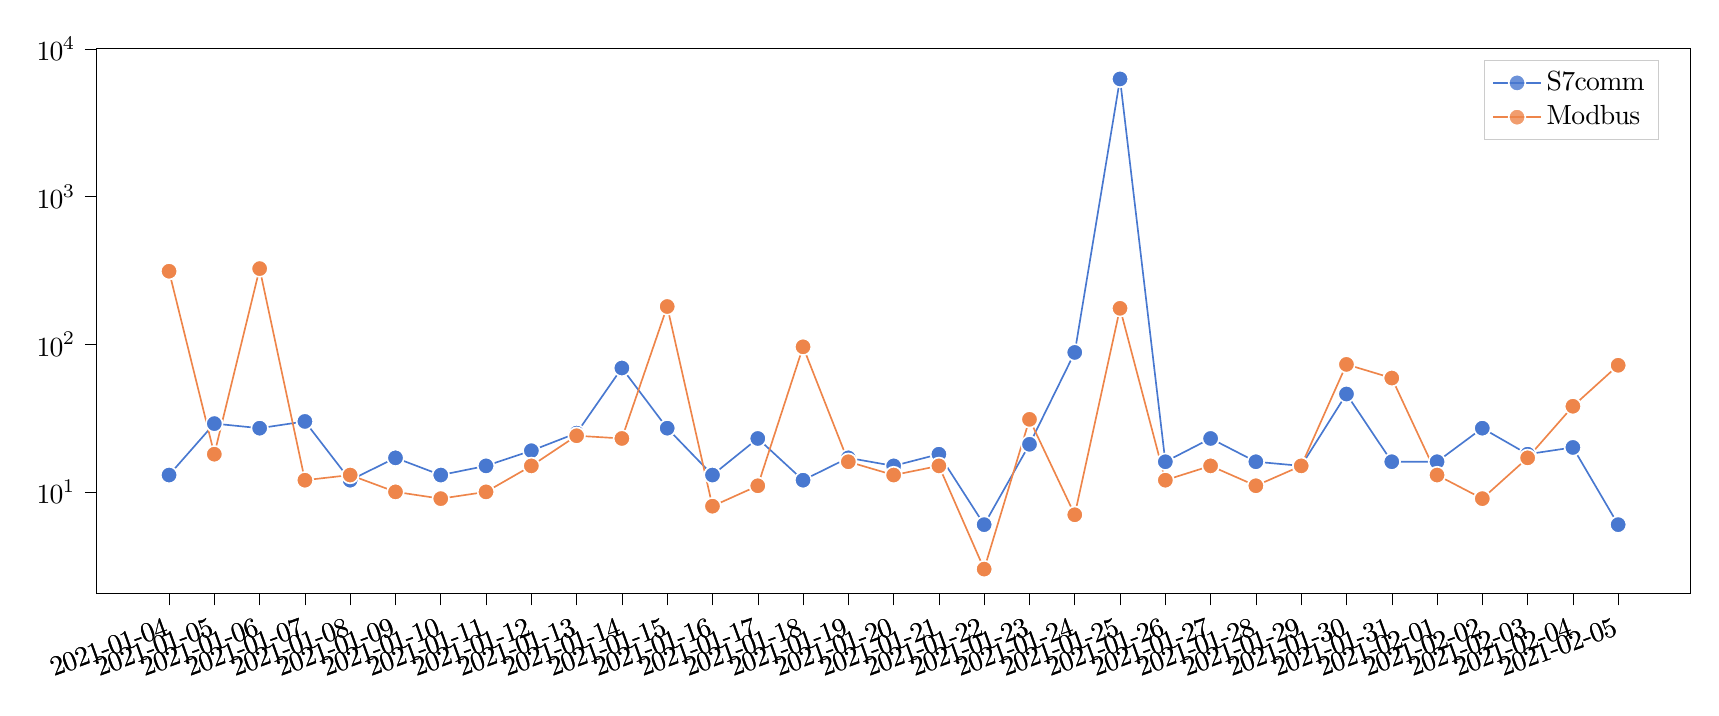
\begin{tikzpicture}
		
		\definecolor{color0}{rgb}{0.282352941176471,0.470588235294118,0.815686274509804}
		\definecolor{color1}{rgb}{0.933333333333333,0.52156862745098,0.290196078431373}
		
		\begin{axis}[
		legend cell align={left},
		legend style={fill opacity=0.8, draw opacity=1, text opacity=1, draw=white!80!black},
		log basis y={10},
		scaled x ticks = false,
		tick align=outside,
		tick pos=left,
		x grid style={white!69.0196078431373!black},
		xmin=737792.4, xmax=737827.6,
		xtick style={color=black},
		xtick={737794,737794,737795,737795,737796,737796,737797,737797,737798,737798,737799,737799,737800,737800,737801,737801,737802,737802,737803,737803,737804,737804,737805,737805,737806,737806,737807,737807,737808,737808,737809,737809,737810,737810,737811,737811,737812,737812,737813,737813,737814,737814,737815,737815,737816,737816,737817,737817,737818,737818,737819,737819,737820,737820,737821,737821,737822,737822,737823,737823,737824,737824,737825,737825,737826,737826},
		xticklabel style={rotate=20.0,anchor=north east},
		xticklabels={
			2021-01-04,
			2021-01-04,
			2021-01-05,
			2021-01-05,
			2021-01-06,
			2021-01-06,
			2021-01-07,
			2021-01-07,
			2021-01-08,
			2021-01-08,
			2021-01-09,
			2021-01-09,
			2021-01-10,
			2021-01-10,
			2021-01-11,
			2021-01-11,
			2021-01-12,
			2021-01-12,
			2021-01-13,
			2021-01-13,
			2021-01-14,
			2021-01-14,
			2021-01-15,
			2021-01-15,
			2021-01-16,
			2021-01-16,
			2021-01-17,
			2021-01-17,
			2021-01-18,
			2021-01-18,
			2021-01-19,
			2021-01-19,
			2021-01-20,
			2021-01-20,
			2021-01-21,
			2021-01-21,
			2021-01-22,
			2021-01-22,
			2021-01-23,
			2021-01-23,
			2021-01-24,
			2021-01-24,
			2021-01-25,
			2021-01-25,
			2021-01-26,
			2021-01-26,
			2021-01-27,
			2021-01-27,
			2021-01-28,
			2021-01-28,
			2021-01-29,
			2021-01-29,
			2021-01-30,
			2021-01-30,
			2021-01-31,
			2021-01-31,
			2021-02-01,
			2021-02-01,
			2021-02-02,
			2021-02-02,
			2021-02-03,
			2021-02-03,
			2021-02-04,
			2021-02-04,
			2021-02-05,
			2021-02-05
		},
		y grid style={white!69.0196078431373!black},
		ymin=2.04721040620367, ymax=10000,
		ymode=log,
		ytick style={color=black},
		ytick={10,100,1000,10000},
		yticklabels={
			\(\displaystyle {10^{1}}\),
			\(\displaystyle {10^{2}}\),
			\(\displaystyle {10^{3}}\),
			\(\displaystyle {10^{4}}\)
		}
		]
		\addplot [semithick, color0, mark=*, mark size=3, mark options={solid,draw=white}]
		table {%
			737794 13
			737795 29
			737796 27
			737797 30
			737798 12
			737799 17
			737800 13
			737801 15
			737802 19
			737803 25
			737804 69
			737805 27
			737806 13
			737807 23
			737808 12
			737809 17
			737810 15
			737811 18
			737812 6
			737813 21
			737814 88
			737815 6256
			737816 16
			737817 23
			737818 16
			737819 15
			737820 46
			737821 16
			737822 16
			737823 27
			737824 18
			737825 20
			737826 6
		};
		\addlegendentry{S7comm}
		\addplot [semithick, color1, mark=*, mark size=3, mark options={solid,draw=white}]
		table {%
			737794 312
			737795 18
			737796 325
			737797 12
			737798 13
			737799 10
			737800 9
			737801 10
			737802 15
			737803 24
			737804 23
			737805 180
			737806 8
			737807 11
			737808 96
			737809 16
			737810 13
			737811 15
			737812 3
			737813 31
			737814 7
			737815 175
			737816 12
			737817 15
			737818 11
			737819 15
			737820 73
			737821 59
			737822 13
			737823 9
			737824 17
			737825 38
			737826 72
		};
		\addlegendentry{Modbus}
		\end{axis}
		\end{tikzpicture}
		
	\end{adjustbox}
	\caption{Evolution of ICS events over time recorded between January and February 2021, comparing S7comm and Modbus.}
	\label{fig:evo_ics}
\end{figure*}


We grouped the activities relating to ICS services to then represent their temporal evolution.
To do this, we loaded the log of the generic connections obtained through Zeek towards Elasticsearch, pivoting the data into a new service-centric index.
The table generated in this way was exported and expressed graphically via time series.
In Figure~\ref{fig:evo_ics} we notice that on some days there is a positive correlation between the events of the two services, while in some other days there is not.
On January 25 there was a relevant increase in requests towards S7comm, while we can record more lesser peaks concerning Modbus. Given such a correlation, it is useful to analyze data in deep and identify the most active hosts that made requests to either S7comm or Modbus, and to both of them. 

\begin{figure}[htb]
	\centering
	\begin{adjustbox}{width=0.46\textwidth}
		% This file was created by tikzplotlib v0.9.8.
		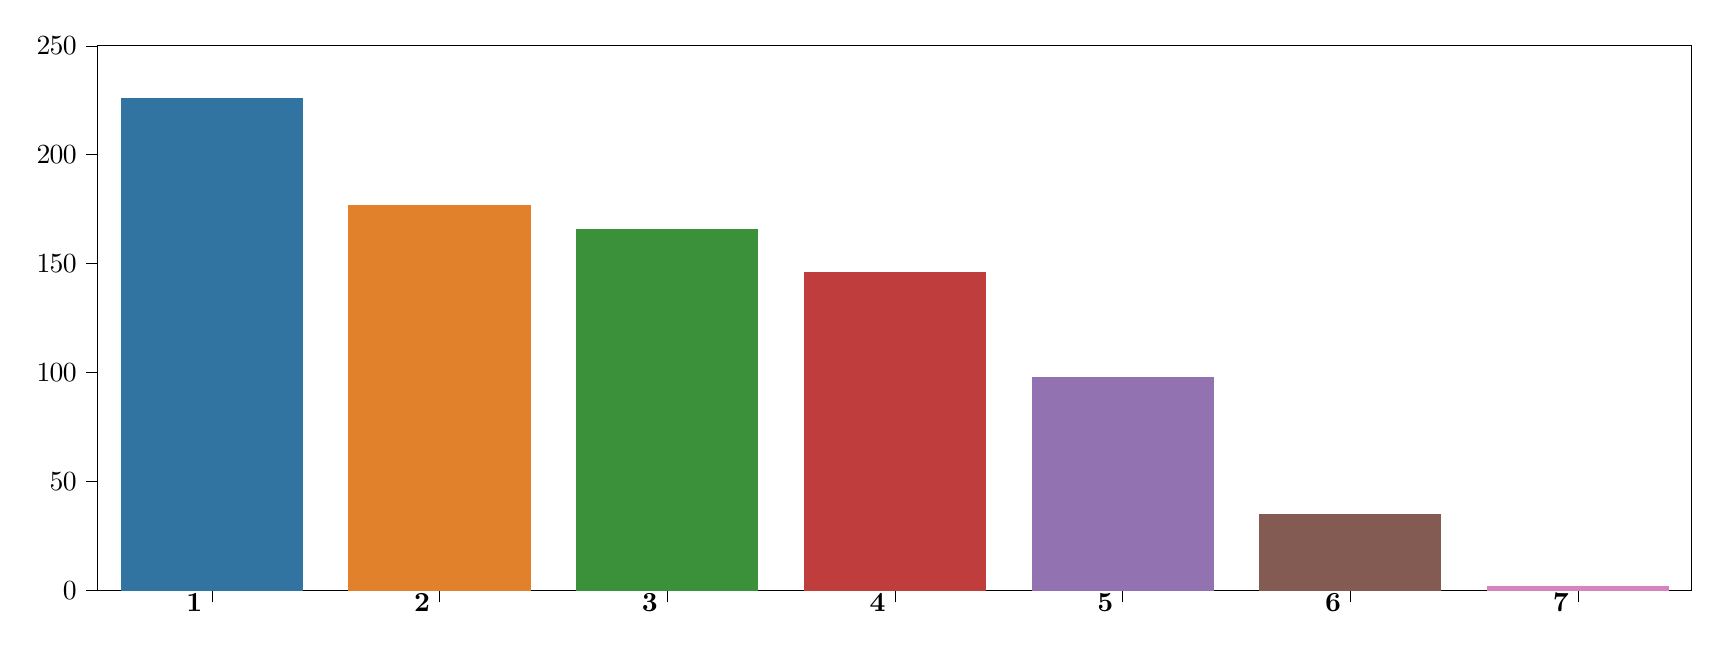
\begin{tikzpicture}
		
		\definecolor{color0}{rgb}{0.194607843137255,0.453431372549019,0.632843137254902}
		\definecolor{color1}{rgb}{0.881862745098039,0.505392156862745,0.173039215686275}
		\definecolor{color2}{rgb}{0.229411764705882,0.570588235294118,0.229411764705882}
		\definecolor{color3}{rgb}{0.75343137254902,0.238725490196078,0.241666666666667}
		\definecolor{color4}{rgb}{0.578431372549019,0.446078431372549,0.699019607843137}
		\definecolor{color5}{rgb}{0.517156862745098,0.358333333333333,0.325980392156863}
		\definecolor{color6}{rgb}{0.837254901960784,0.519607843137255,0.740196078431372}
		
		\begin{axis}[
		tick align=outside,
		tick pos=left,
		x grid style={white!69.0196078431373!black},
		xmin=-0.5, xmax=6.5,
		xtick style={color=black},
		xtick={0,1,2,3,4,5,6},
		xticklabel style={rotate=0.0,anchor=east,font=\HUGE, font=\bf},
		xticklabels={
			1,
			2,
			3,
			4,
			5,
			6,
			7
		},
		y grid style={white!69.0196078431373!black},
		ymin=0, ymax=250,
		ytick style={color=black}
		]
		\draw[draw=none,fill=color0] (axis cs:-0.4,0) rectangle (axis cs:0.4,226);
		\draw[draw=none,fill=color1] (axis cs:0.6,0) rectangle (axis cs:1.4,177);
		\draw[draw=none,fill=color2] (axis cs:1.6,0) rectangle (axis cs:2.4,166);
		\draw[draw=none,fill=color3] (axis cs:2.6,0) rectangle (axis cs:3.4,146);
		\draw[draw=none,fill=color4] (axis cs:3.6,0) rectangle (axis cs:4.4,98);
		\draw[draw=none,fill=color5] (axis cs:4.6,0) rectangle (axis cs:5.4,35);
		\draw[draw=none,fill=color6] (axis cs:5.6,0) rectangle (axis cs:6.4,2);
		\end{axis}
		\end{tikzpicture}
		
	\end{adjustbox}
	\caption{Modbus requests received: 1) Read Device Identification, 2) Unknown-218, 3) Read Holding Register, 4) Report Slave ID, 5) Write Multiple Registers, 6) Write Multiple Registers Exception, 7) Read Input Register Exception.}
	\label{fig:modbus_fc}
\end{figure}

Figure~\ref{fig:modbus_fc} shows the number and type of Modbus requests we logged in one month.
The most frequent event is \emph{Read Device Identification}, which is invoked using function code 43.
This encapsulation mechanism allows to transfer predefined and reserved fields: reserved function codes are implemented by companies and are not available for public use.
In addition to being a field that is commonly read by search engines, it also corresponds to the first stage (i.e., planning) of the \emph{ICS killchain}~\cite{killchain}.
This stage is usually conducted both actively using reconnaissance tools, and passively through
search engines such as Shodan or other services that allow for investigating the targeted resource without interacting directly with it. 

We were able to detect the stealth scans, identifed with the Unknown-218 exception. In fact, using Wireshark we identified this kind of activity by following the \emph{SYN $\rightarrow$ SYN/ACK $\rightarrow$ RST} pattern.
This type of request, as we also see in  Table~\ref{tab:modbus_actors}, was always performed by scanners and we believe it is therefore a benign request.

We logged unauthorized reading requests to the \emph{holding registers}, which  store 16 bits readable and writable configuration-values. 
There are also exceptions related to the reading of input registers (i.e., $16$ bits values representing measurements and statuses). 
We believe that a host has tried to access an undefined input, i.e. the register does not exist. 
Similarly, the same holds true for \emph{Write Multiple Registers} exceptions.
We detected many requests for writing to multiple registers,
where unauthenticated hosts attempted to corrupt the honeypot, or were looking for some undefined behavior of our configuration.


\begin{figure}[htb]
	\centering
	\begin{adjustbox}{width=0.46\textwidth}
		% This file was created by tikzplotlib v0.9.8.
		
		% This file was created by tikzplotlib v0.9.8.
		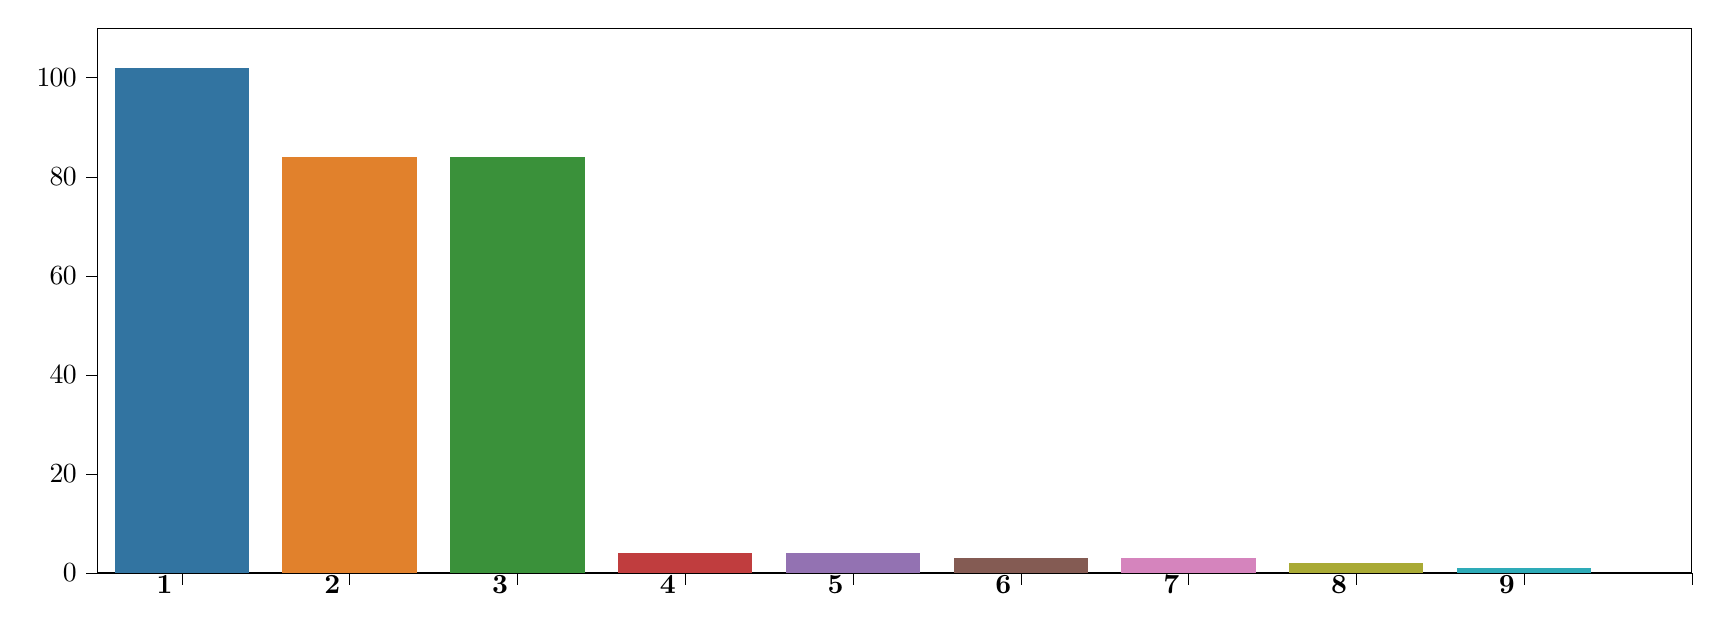
\begin{tikzpicture}
		
		\definecolor{color0}{rgb}{0.194607843137255,0.453431372549019,0.632843137254902}
		\definecolor{color1}{rgb}{0.881862745098039,0.505392156862745,0.173039215686275}
		\definecolor{color2}{rgb}{0.229411764705882,0.570588235294118,0.229411764705882}
		\definecolor{color3}{rgb}{0.75343137254902,0.238725490196078,0.241666666666667}
		\definecolor{color4}{rgb}{0.578431372549019,0.446078431372549,0.699019607843137}
		\definecolor{color5}{rgb}{0.517156862745098,0.358333333333333,0.325980392156863}
		\definecolor{color6}{rgb}{0.837254901960784,0.519607843137255,0.740196078431372}
		\definecolor{color7}{rgb}{0.662254901960784,0.665196078431373,0.209313725490196}
		\definecolor{color8}{rgb}{0.180392156862745,0.67156862745098,0.72156862745098}
		
		\begin{axis}[
		tick align=outside,
		tick pos=left,
		x grid style={white!69.0196078431373!black},
		xmin=-0.5, xmax=9,
		xtick style={color=black},
		xtick={0,1,2,3,4,5,6,7,8,9},
		xticklabel style={rotate=0.0,anchor=east,font=\large, font=\bf},
		xticklabels={
			{1},
			{2},
			{3},
			{4},
			{5},
			{6},
			{7},
			{8},
			{9} 
		},
		y grid style={white!69.0196078431373!black},
		ymin=0, ymax=110,
		ytick style={color=black}
		]
		\draw[draw=none,fill=color0] (axis cs:-0.4,0) rectangle (axis cs:0.4,102);
		\draw[draw=none,fill=color1] (axis cs:0.6,0) rectangle (axis cs:1.4,84);
		\draw[draw=none,fill=color2] (axis cs:1.6,0) rectangle (axis cs:2.4,84);
		\draw[draw=none,fill=color3] (axis cs:2.6,0) rectangle (axis cs:3.4,4);
		\draw[draw=none,fill=color4] (axis cs:3.6,0) rectangle (axis cs:4.4,4);
		\draw[draw=none,fill=color5] (axis cs:4.6,0) rectangle (axis cs:5.4,3);
		\draw[draw=none,fill=color6] (axis cs:5.6,0) rectangle (axis cs:6.4,3);
		\draw[draw=none,fill=color7] (axis cs:6.6,0) rectangle (axis cs:7.4,2);
		\draw[draw=none,fill=color8] (axis cs:7.6,0) rectangle (axis cs:8.4,1);
		\end{axis}
		
		\end{tikzpicture}
		
	\end{adjustbox}
	\caption{S7comm requests received: 1) Setup Communication, 2) Read SZL ID: 0x001c index: 0x0001, 3) Read SZL ID: 0x0011 index: 0x0001, 4) Read SZL ID: 0x001c index: 0x0000, 5) Read SZL ID: 0x0011 index: 0x0000, 6) Read SZL ID:0x0011 index: 0x0000, 7) Read SZL ID:0x0232 index: 0x0004 8) PLC Stop, 9) Write Variable.}
	\label{fig:s7comm_fc}
\end{figure}


Figure~\ref{fig:s7comm_fc} concerns S7comm events instead. We collected a large number of \emph{Setup Communication requests}, used to establish a communication with the S7comm Layer. 
We found a significant number of \emph{READ SZL} requests, split in five different request parameters. 
This function code is used to read the system status. 
By using Wireshark, we noticed that the requests captured are similar to the \emph{s7-info.nse script}, 
used for functions coverage during the local testing phase of our solution. The same behavior was also confirmed in \emph{ENISA}.\footnote{The European Union Agency for Cybersecurity (ENISA): \url{https://www.enisa.europa.eu/topics/trainings-for-cybersecurity-specialists/online-training-material/documents/introduction-to-network-forensics-ex1-toolset.pdf}.}
Being able to query different fields in \emph{Read SZL} requests, the attacker could be then encouraged to execute other following function codes: a medium-interaction honeypot inactivates possible attackers.
In fact we were able to capture a \emph{PLC Stop (0x29)} request and a \emph{Write (0x05)} variable request on Data Block 1, which respectively stops the CPU and creates a boolean variable assigning it to true.

Given the enormous amount of source hosts, Table~\ref{tab:modbus_actors} and Table~\ref{tab:s7comm_actors}
group host requests by organization and the corresponding \emph{Autonomous System Number} (\emph{ASN}). 

Most of the requests are harmless and end with the information gathering phase performed on both services. 
Among the actors who carried out these requests we identified \emph{Censys} and \emph{CARI.net} (the owner of Shodan IP addresses).
However, there are organizations that have made malicious requests to our services.
\emph{M247} made unsuccessful requests to the Modbus protocol. We believe that the actor had first passively inquired through a search engine,
and that he expected certain registers to be initialized. 
On the other hand, M247 had a more linear behavior towards the S7comm service, 
starting primarily from the reconnaissance phase actively carried out. 
Only after this stage did it perform malicious activities such as attempting to tamper with the CPU as shown in Table~\ref{tab:s7comm_actors}. 

The main source of malicious requests is \emph{Pacswitch}, where the host has compromised both services in a sharp way.
Unlike the host belonging to M247, the activities of this actor were also actively carried out in the initial phase with a chronologically linear attack stage.
In the case of Modbus, the actor overwrote all existing registers, also attempting to overwrite nonexistent registers.
We believe the actor used a script or a framework such as SMOD\footnote{https://github.com/theralfbrown/smod-1.} capable of bruteforce against all the registers. 
As for the S7comm service, Pacswitch was the only host to perform two particular write and read requests. 
Thanks to our honeypot we managed to specifically identify the read request \emph{SZL ID: 0x0232 index: 0004}.
As illustrated by the reference manual, this partial list contains various information about the CPU,
among which we mention its protection level, and the position of the operating mode selector (CRST/WRST\footnote{In CRST mode, the data present are deleted and the program parameters are reinitialized.}).
The same actor performed a write variable request that lasted 7 seconds, sending 83 bytes in input. 
With this request the actor created an unrecognized boolean tag in Data Block 1 set to True. 


\begin{table}[htb]
	\centering
	\scalebox{0.9}{
	\begin{tabular}{lllllllll}
		\hline
		\textbf{Organization} & \textbf{ASN} & 
		\rotation{0}{1} & 
		\rotation{0}{2} & 
		\rotation{0}{3} & 
		\rotation{0}{4} & 
		\rotation{0}{5} &
		\rotation{0}{6} &
		\rotation{0}{7}\\
		Pacswitch & 55536 & & \cmark & \cmark & \cmark & \cmark & \cmark & \\
		M247 & 9009 & & & & \cmark & & & \cmark \\
		IP Volume & 202425 & \cmark & & & & & & \cmark \\
		CARI.net & 10439 & \cmark & & & & & & \cmark \\
		DigitalOcean & 14061 & & \cmark & & & & & \\
		Censys & 398705 & & \cmark & & & & & \\
		SOFTLAYER & 36351 & & \cmark & & & & & \\
		Merit & 237 & & \cmark & & & & & \\
		Leaseweb & 60781 & & \cmark & & & & & \\
		CT-Hangzou-IDC & 58461 & & \cmark & & & & & \\
		ZNET & 21859 & & \cmark & & & & & \\
		Novogara LTD & 204655 & & \cmark & & & & & \\
		CDSC-AS1 & 63199 & \cmark & \cmark & & & & & \\
		Unmetered & 54133 & & & & & & & \cmark \\
		OVH & 16276 & & \cmark & & & & & \\
		Eonix & 62904 & & \cmark & & & & & \\
		ChinaNet & 38283 & & \cmark & & & & & \\
		OPI-NET-LTD & 206776 & & \cmark & & & & & \\
		China Mobile & 9808 & & \cmark & & & & & \\
		Alpha Strike & 208843 & & \cmark & & & & & \\
	\end{tabular}
}
	\caption{Modbus request types corresponding to the organization: 1) Report Slave ID, 2) Read Device Identification, 3) Read Holding Register, 4) Read Input Register Exception, 5) Write Multiple Registers, 6) Write Multiple Registers Exception, 7) Unknown-218.}
	\label{tab:modbus_actors}
\end{table}


\begin{table}[htb]
	\centering
	\scalebox{0.9}{
	\begin{tabular}{llllllllll}
		\hline
		\textbf{Organization} & \textbf{ASN} & 
		\rotation{0}{1} & 
		\rotation{0}{2} & 
		\rotation{0}{3} & 
		\rotation{0}{4} & 
		\rotation{0}{5} &
		\rotation{0}{6} &
		\rotation{0}{7} &
		\rotation{0}{8} \\
		DigitalOcean & 14061 & \cmark & \cmark & \cmark & \cmark & \cmark & & \\
		Censys & 398705 & \cmark & \cmark & \cmark & \cmark & \cmark & & & \\
		CARI.net & 10439 & \cmark & \cmark & & \cmark & & & &\\
		IP Volume & 202425 & \cmark & \cmark & \cmark & \cmark & & & \\
		M247 & 9009 & \cmark & \cmark & & \cmark & & & \cmark &\\
		Pacswitch & 55536 & \cmark & & \cmark & & \cmark & \cmark & & \cmark \\
		GleSYS AB & 42708 & \cmark & \cmark & & \cmark & & & & \\
		SOFTLAYER & 36351 & & \cmark & & & & & & \\
		Cogent & 174 & \cmark & \cmark & & & & & & \\
		Merit & 237 & \cmark & \cmark & & \cmark & & &\\
		Bluecloud & 58593 & \cmark & & & & & & & \\
		Alpha Strike & 208843 & \cmark & \cmark & & \cmark & & & & \\
		OVH & 16276 & \cmark & & & & & & & \\
	\end{tabular}}
	\caption{S7comm request types corresponding to the organization: 1) Setup Communication, 2) Read SZL ID: 0x001c index: 0x0001, 3) Read SZL ID: 0x001c index: 0x0000, 4) Read SZL ID: 0x0011 index: 0x0001, 5) Read SZL ID: 0x0011 index: 0x0000, 6) Read SZL ID: 0x0232 index: 0x0004, 7) PLC Stop, 8) Write Variable.}
	\label{tab:s7comm_actors}
	
\end{table}

\iffalse
Setup comm = 1
id=0x001c index=0001 = 2
id=0x001c index=0000 = 3
id=0x0011 index=0001 = 4
id=0x0011 index=0000 = 5
0x0232 index:0x0004 = 6
Stop CPU = 7
Write Var = 8
\fi

\begin{remark}\label{rmk:syn}
	In Figure~\ref{fig:s7comm_fc} we report all the activities of the S7comm application layer.
	We found that the the peak of activities recorded on January 25 2021 towards port 102 was mostly due to TCP SYN scans.
	This was discovered thanks to the separation of logs by protocol type: in that one related to the application layer
	there was no trace of the performed-request TYPE. 
	However, by crossing the such a log with the one related to the activities recorded in the presentation layer (ISO-COTP), we realized
	a high number of half-open connections\footnote{The lack of synchronization could be due to malicious intent, such as the TCP SYN Flood attack.}
	were recorded by the same actor having unknown DNS assigned to IP Volume inc. (ASN 202425). 
	This host carried out this activity without actively obtaining information about our instance.
	We believe that the host already knew our configuration thanks to search engines like Censys. 
\end{remark}

Table~\ref{tab:req_class} shows the number of logged activities classified as benign or malicious. From the total number of activities we removed TCP SYN scans, as described in Rmk.~\ref{rmk:syn}.
With reference to the Modbus service we classified as benign ``Report Slave Id'', ``Read device identification'' and ``Unknown-218'' requests.
Instead, we considered reading requests other than those indicated above as intrusive such as the reading of coils and registers that may contain confidential information. 
We considered read requests to the S7comm protocol, with the exception of those that concern the CPU protection level,
as benign, since they are mostly performed by periodic scanners. 
Any S7comm write request, including exceptions, was clearly treated as malicious, regardless of the service.


\begin{table}[htb]
	\centering
	\begin{tabular}{c|c|c}
		
		& \textbf{Modbus} & \textbf{S7comm}\\ \hline
		\textbf{Benign} & 549 & 274 \\ \hline
		\textbf{Malicious} & 301 & 6 \\ \hline

	\end{tabular}
	\caption{Number of logged activities based on their benign or malicious nature, and not considering TCP SYN scans.}
	\label{tab:req_class}
\end{table}

The high number of Modbus requests classified as malicious can be
explained by the fact that \emph{i)} the interaction with a Modbus PLC, by design, can involve multiple coils and registers, 
and \emph{ii)} Modbus is now an open standard (unlike S7comm), which makes it easier to write a script that brute-forces against all the registers.




\section{Behavior of Attackers}\label{sec:behavior}
In order to characterize the attacker profile, in this section we consider the data represented in Figure~\ref{fig:evo_ics} and we outline its sequence of commands (i.e., the host behavior) grouped by IP address.

For each host, the sequence of commands executed was captured only once, and there were no recurring activities from the same IP during the high-intensity periods. 
We discovered this by grouping events initially by a certain time slot, and subsequently by day, noting that the sequence of commands remained unchanged.
We believe this is due to the duration of the experiment, as in general the port scanners  repeat the same activities on a monthly basis. 

We represented the encoded sequence of commands for hosts related to Modbus requests. 
We consider 5 of these command patterns  as relevant, and we show them in Table~\ref{tab:commseq_mod}, where the apex on each command represents the number of logged repetitions in sequence.  Each of these patterns (P) was  logged on a different day, as reported by Table~\ref{tab:commseq_mod}.

\begin{table}[h]
	\centering 
	\scalebox{0.85}{
		\begin{tabular}{ccccc}
			\hline
			& \textbf{IP}  & \textbf{ASN} & \textbf{Organization} & \textbf{Pattern}\\ \hline\\
			\textbf{P1}  & 27.122.12.245 & 55536 & Pacswitch & 2, 0, 1\textsuperscript{84}, 4, 5\textsuperscript{33}, 1\textsuperscript{82} \\
			\textbf{P2} & 185.104.184.99 & 9009 & M247 & 2, 0, 6\textsuperscript{160}\\
			\textbf{P3} & 93.174.95.106  & 29073 & IP Volume& 3, 0, 6\textsuperscript{3}, 3, (0, 3)\textsuperscript{38}\\
			\textbf{P4}  & 71.6.199.23 & 10439 & CARI.net & 3, 0, 6\textsuperscript{3}, (3, 0)\textsuperscript{14}\\
			\textbf{P5} & 71.6.146.185 & 10439  & CARI.net & 3, 0, 6\textsuperscript{3}, (3, 0)\textsuperscript{15}\\ \hline
		\end{tabular}}
	\caption{Host sequence of commands related to Modbus service. The daily periods analyzed are: P1) January 6, P2) January 15, P3) January 25, P4) January 30, P5) February 5.
		The events are mapped as follows : 0) Read Device Identification, 1) Read Holding Registers, 2) Read Input Registers Exception,
		3) Report Slave ID, 4) Write Multiple Registers, 5) Write Multiple Registers Exception, 6) Unknown-218 (Half-open scan). The apex on each command represents the number of logged repetitions in sequence.}
	\label{tab:commseq_mod}
\end{table}




We can clearly distinguish the recurring scanners with the harassing actors during the initial phase of communication.
The actors belonging to the CARI.net and IP Volume organization have an almost identical behavior, and start their activity by making Report Slave ID and Read Device Identification requests.
We could remove the first two commands, as typically a couple of read requests (slave and device information) are needed to know how to compromise the device.
But as we can see in Table~\ref{tab:commseq_mod}, this is not true.
In fact, M247 and Pacswitch hosts execute Read Device Identification request only after making an illegal reading of the registers (note that M247 performed 160 TCP SYN requests, which may indicate a suspicious behavior). 

For what concerns the activities towards the S7comm protocol, we identified in a similar way the most interesting patterns during the periods of greatest intensity.
Differently to what emerged with  Modbus activities, very similar S7comm patterns were recorded belonging to hosts of the same organization.
Moreover, some actors performed the exact same sequence during the period of intense activity. 
In order to simplify the representation, we assume with regard to the S7comm activities, that the hosts of an Autonomous System have the same behavior. 
In Table~\ref{tab:commseq_s7} we represent the sequence of commands performed by Organization hosts, grouped by high-intensity activity period.

\begin{table}[h]
	\centering 
	\scalebox{0.85}{
		\begin{tabular}{ccccc}
			\hline
			& \textbf{IP}  & \textbf{ASN} & \textbf{Organization} & \textbf{Pattern}\\ \hline
			\textbf{P1} & \makecell{167.248.133.37, \\ 89.248.174.3} & \makecell{398722, \\ 202425}  & Censys, IP Volume & 8, 2, 4, 5, 4, 5 \\
			\textbf{P2} & 27.122.12.245 & 55536 & Pacswitch & 8, 2, 9, 3 \\
			%\textbf{P3} & 89.248.174.3 & 202425 & IP Volume & - \\
			\textbf{P3} & 192.241.222.191 & 14061 & DigitalOcean & 8, 2, 4, 5, 4, 5 \\ \hline
			
	\end{tabular}}
	\caption{Host sequence of commands related to S7comm service. The daily periods analyzed are: P1) January 14 and January 24, P2) January 24, P3) January 30.
		The events are mapped as follows: 2) Setup Communication response, 3) Write variable reponse, 4) Read SZL request, 5) Read SZL response,  8) Setup Communication request, 9) Write variable request. the apex on each command represents the number of logged repetitions in sequence.}
	\label{tab:commseq_s7}
\end{table}

Regarding the S7comm service, we were able to reconstruct the complete communication between the actors and the honeypot,
reporting in chronological order the response to each request made.
As the results show, DigitalOcean hosts that make two Read SZL requests followed by the Setup Communication request are recurring scanners.
The behavior of the Pacswitch host differs from the aforementioned host, 
which instead of running a portscan tries to write directly to our honeypot. 
The unrecognized pattern of the host belonging to IP Volume inc. is explained in  Remark~\ref{rmk:syn}.









\section{Conclusion and Future Works}\label{sect:conclusion}
We presented LOGistICS, a multi-component framework where to study the security of ICSs. 
The core of the system is represented by a new medium-interaction honeypot modeling Modbus and S7comm respectively.
These protocols are among the most used in industrial PLC. The paper focuses on this honeypot, which are shown to be less detectable by attackers than similar proposals, and indistinguishable from real PLCs when using automated attack-tools (e.g., Metasploit/ISF).
Finally, we tested how LOGistICS works by exposing it to the Internet for one month. 
We found that most of the requests made are not malicious. 
However, the hosts making such requests do not have the same behavior, which differs in the type of information they read. 
Moreover, we found that besides periodic scanners (e.g. Shodan and Censys) who conclude their activity once the reconnaissance stage has been completed,
there exist attacks trying to write data and control the PLC.

From what accomplished we collected several ideas about possible extensions as future work. For instance, we would like to use ELK as a SIEM.
The aim is to leave the honeypot always running, and monitor live data-streams. 
In this way, it is possible to provide real-time analysis of security alerts. In this paper we were interested in an off-line study though.

We would like to better assess and improve the undetectability of the honeypot components of LOGistICS, in particular the S7comm one.
From what computed by Honeyscore, it has a low probability of being undetected but still greater than zero.
A possible approach we intend to take is to implement technologies that can emulate TCP/IP fingerprinting through host device emulation on a virtual network. 
Moreover, we could emulate additional services that are typical of network-exposed PLCs, as for example SNMP, with the purpose to deceive scanners and attackers.

In addition, besides improving the extensibility end configurability of the honeypot already offered, 
in the future we would like to use additional deception-technology components: 
for example, we want to add protocols as \emph{i)} \emph{BACnet} (\emph{Building Automation and Control}), 
which finds its application in ventilating, heating, access control, lightning, air-conditioning and fire detection systems; 
and \emph{ii}) \emph{DNP3} (\emph{Distributed Network Protocol}), which is is widely adopted in theUSA and Canada,
and it is used by electric and water companies.






 


\section*{Acknowledgments}
We would like to thank Davide Nardella for the help provided with the interpretation of fields in the Snap7 firmware.


\FloatBarrier


\bibliographystyle{elsarticle-num}
\bibliography{biblio}

\section*{Appendix}
In the following of the Appendix we report additional  templates in LOGistICS, implementing the behavior of further ICS devices.

\begin{lstlisting}[basicstyle=\scriptsize,label={lst:s7_300_template},float=htb,caption={Simatic S-300 honeypot template scanned using s7-info NSE script.}, captionpos=b,breaklines=true]

102/tcp open  iso-tsap
| s7-info: 
|   Module: 6ES7 314-1AF10-0AB0 
|   Basic Hardware: 6ES7 314-1AF10-0AB0 
|   Version: 3.2.6
|   System Name: SIMATIC S-300
|   Module Type: CPU 314C-2 DP
|   Serial Number: 46202011
|_  Copyright: Original Siemens EquipmentS C-B6UT46202011
\end{lstlisting}

\begin{lstlisting}[basicstyle=\scriptsize,label={lst:s7_1200_template},float=htb,caption={Simatic S-1200 honeypot template scanned using s7-info NSE script.}, captionpos=b,breaklines=true]
102/tcp open  iso-tsap
| s7-info: 
|   Module: 6ES7 214-1AG40-0XB0 
|   Basic Hardware: 6ES7 214-1AG40-0XB0 
|   Version: 3.2.6
|   System Name: SIMATIC S-1200
|   Module Type: CPU 1214C
|   Serial Number: S C-C2UR28722014
|_  Copyright: Original Siemens Equipment
\end{lstlisting}


\begin{lstlisting}[basicstyle=\scriptsize,label={lst:toshiba},float=htb,caption={Toshiba PLC template scanned using modbus-discover NSE script.}, captionpos=b,breaklines=true]
502/tcp open  modbus
| modbus-discover: 
|   sid 0x1: 
|     Slave ID data: Toshiba-38883775847289-1.3\xFF
|_    Device identification: Toshiba 38883775847289 1.3
\end{lstlisting}


\begin{lstlisting}[basicstyle=\scriptsize,label={lst:beckhoff},float=h,caption={Beckhoff PLC template scanned using modbus-discover NSE script.}, captionpos=b,breaklines=true]
502/tcp open  modbus
| modbus-discover: 
|   sid 0x1: 
|     Slave ID data: Beckhoff-3917C8160000-3.1\xFF
|_    Device identification: Beckhoff 3917C8160000 3.1
\end{lstlisting}

\begin{lstlisting}[basicstyle=\scriptsize,label={lst:panasonic},float=h,caption={Panasonic PLC template scanned using modbus-discover NSE script.}, captionpos=b,breaklines=true]
502/tcp open  modbus
| modbus-discover: 
|   sid 0x1: 
|     Slave ID data: Panasonic-13559727101-4.52\xFF
|_    Device identification: Panasonic 13559727101 4.52
\end{lstlisting}






\end{document}
